\documentclass[3p]{elsarticle}
\usepackage[english]{babel}
\usepackage{amsmath,amssymb}
\usepackage{amsthm}
\usepackage{thmtools, thm-restate}
\usepackage{breqn}
\usepackage{bbold}
\usepackage{booktabs}
\usepackage{graphicx}
\usepackage[utf8]{inputenc}
\usepackage[T1]{fontenc}
\usepackage{caption}
\usepackage{siunitx}
\usepackage{hyperref}
\usepackage[labelfont=bf,textfont={sl,bf},lofdepth,lotdepth]{subfig}
\usepackage{xspace}
\usepackage{color}
\usepackage{proba}
\usepackage[usenames,dvipsnames,svgnames,table]{xcolor}
\usepackage{cleveref}
\usepackage{paralist}
\usepackage{todonotes}
\usepackage{bigints}
\usepackage[title,titletoc,toc]{appendix}
\usepackage{import}
\usepackage{natbib}
%%%%%%%%%%%%%%%%%%%%%%%%%%%%%%%%%%%%%%%%%%%%%%%%%%%%%%%%%%%%%%%%%%%%%%%%%%%%%%%%%%%%%%%%%%
%                                  MODIFICACIONES                                        %
%%%%%%%%%%%%%%%%%%%%%%%%%%%%%%%%%%%%%%%%%%%%%%%%%%%%%%%%%%%%%%%%%%%%%%%%%%%%%%%%%%%%%%%%%%
\oddsidemargin=1.0cm
%\evensidemargin=2.0cm
\textwidth=14.5cm
%%%%%%%%%%%%%%%%%%%%%%%%%%%%%%%%%%%%%%%%%%%%%%%%%%%%%%%%%%%%%%%%%%%%%%%%%%%%%%%%%%%%%%%%%%
%                                 FORMATOS                                               %
%%%%%%%%%%%%%%%%%%%%%%%%%%%%%%%%%%%%%%%%%%%%%%%%%%%%%%%%%%%%%%%%%%%%%%%%%%%%%%%%%%%%%%%%%%
%\DeclareMathAlphabet{\mathpzc}{OT1}{pzc}{m}{it}
\theoremstyle{definition}
\newtheorem{definition}{Definition}[section]
\newtheorem{dfn}{Definition}[section]
\newtheorem{assumption}{Assumption}[section]
\newtheorem{hypothesis}{Hypothesis}[section]
%
\theoremstyle{plain}% default
\newtheorem{thm}{Theorem}[section]
\newtheorem{pro}{Proposition}[section]
\newtheorem{lem}{Lemma}[section]
\newtheorem{corollary}{Corollary}[section]
\newtheorem{consequence}{CONSEQUENCE}[section]
\newtheorem{example}{\bf Example}[section]
\theoremstyle{remark}
\newtheorem{remark}{Remark}[section]
\newproof{pf}{Proof}

%declaration theorems for appendix
\declaretheorem[numbered=no, name=H\"{o}lder]{Holder}
\declaretheorem[numbered=no, name=Young]{Young}
\declaretheorem[numbered=no, name=Minkowski]{Minkowski}
\declaretheorem[numbered=no, name=Doob's Martingale Inequality]{Doobs}
\declaretheorem[numbered=no, name=Burkholder–Davis–Gundy inequality]{bdg}
\declaretheorem[numbered=no, name=Gronwall inequality]{Gronwall}
\declaretheorem[numbered=no, name=Discrete Gronwall Inequality]{DiscreteGronwall}
\declaretheorem[numbered=no, name=A standard inequality]{Standard}
%
\providecommand*{\lemautorefname}{Lemma}
\providecommand*{\thmautorefname}{Theorem}
\providecommand*{\assumptionautorefname}{Assumption}
\providecommand*{\hypothesisautorefname}{Hypothesis}
\newcommand{\normL}[1]{\left[\mathbb{E}\left|#1\right|^2\right]^{1/2}}
\newcommand{\ms}[1]{\mathbb{E}\left|#1\right|^2}
\newcommand{\mep}[1]{\mathbb{E}|#1|^p}
\newcommand{\m}[1]{\mathbb{E}#1}
\newcommand{\Prob}[1]{\mathbb{P}\left[#1\right]}
\newcommand{\meanp}[2]{\mathbb{E}\left|#1\right|^{#2}}
\newcommand{\condexp}[2]{\mathbb{E}\left[#1|#2\right]}
\newcommand{\lftrght}[3]{\left#2 #1\right #3}\DeclareMathOperator{\tr}{tr}
\newcommand{\innerprod}[2]{\left\langle#1, #2\right\rangle}
\newcommand*{\eg}{e.g.,\xspace}
\newcommand*{\ie}{i.e.,\xspace}
%\newcommand*{\todo}[1]{\textcolor{BrickRed}{#1}\\}
\newcommand{\crefrangeconjunction}{--}
\crefrangeformat{equation}{(#3#1#4)--(#5#2#6)}
\DeclareMathOperator{\diag}{diag}
\DeclareMathOperator*{\as}{a.s.}
%\DeclareMathOperator{\diag}{diag}
\newcommand{\SM}{LS\xspace}
\AtBeginDocument{\renewcommand{\harvardand}{and}}
\declaretheorem[numberwithin=section]{theorem}
%
%+++++++++++++++++++++++++++++++++++++++++++++++++++++++++++++++++++++++++++++++++++++++++++++++++++++++++++++
\begin{document}
	\begin{frontmatter}
		\title{
				Strong Convergence and Almost Sure Stability of the Explicit Linear Steklov Method
				for SDEs under non-globally Lipschitz Coefficients.\tnoteref{t1}
		}%,t2}}
		\tnotetext[t1]{
			This work has been partially
			supported by CONACYT project *****
		}
		\author[sj]{S. D\'{\i}az-Infante}
		\ead{sauld@cimat.mx}
		\author[sj]{S. Jerez}
		\ead{jerez@cimat.mx}
		\address[sj]{Split Step Linear Steklov Method 
		Department of Applied Mathematics, CIMAT, Guanajuato, Gto., Mexico,
		36240.
		}
	\begin{abstract}
		We present an explicit and easily implementable numerical method for
		solving stochastic differential equations (SDEs) with non-globally Lipschitz
		coefficients. A linear version of the Steklov average under a split-step formulation supports our new solver.
		The Linear Steklov (\SM) method converges strongly with a standard 
		one-half order.  Also, we study the almost sure asymptotic stability and in  order to emphasize the 
		performance of the Linear Steklov discretization we use models from population dynamics 
		and non linear stochastic oscillators.
	\end{abstract}
	\begin{keyword}
		stochastic differential equations;
		explicit methods; strong convergence; almost surely asymptotic stability.
	\end{keyword}
	\end{frontmatter}
	%\pagebreak
	%\tableofcontents
	%\pagebreak
	\section{Introduction} 

In this chapter we  study numerical approximations of vector It\^o stochastic differential equations (SDEs) with the 
form
\begin{equation}\label{eqn:SDE1}
	dy(t)
	=f(y(t))dt + g(y(t))dW(t), \quad 0\leq t\leq T,
	\quad y(0)=y_0.
\end{equation}
Here $(f^{(1)},\dots, f^{(d)}):\R^d \to \R^d$ and 
$g = (g^{(i,j)})_{i\in \{1,\dots,d\}, j\in\{1,\dots, m\}}:\R^d \to \R^{d\times m}$.
We will work with the standard setup, that is,  $y(t)\in \R^d$ for each $t$ and  $W(t)$ is a
$m$-dimensional standard Brownian motion on a filtered and complete probability space
$
	(
		\Omega ,\calF,(\calF_t)_{t\in[0,T]},\prob{}
	)
$,
with the filtration
$(\mathcal{F}_t)_{t\in[0,T]}$  generated by the Brownian process.
%
Also, we require the following assumptions over the coefficients 
	$f %= \left(f^{(1)},\dots, 
		%f^{(d)}\right)^{T}
	$,
	$
		g %=(g^{(1)},\ldots g^{(d)})^{T} $, $g^{(j)}:\R^d \to \R^d
	$.
\begin{hypothesis}\label{ass:OSLC}
	The coefficients of SDE \eqref{eqn:SDE1} satisfy the following conditions:
	\begin{enumerate}[({H}-1)]
		\item \label{ass:C1Functions}
		The functions $f,g$ are in the class $C^{1}(\R^d)$.
		\item
		\textbf{Local, global Lipschitz condition}. For each integer $n$, there is a positive
		constant $L_{f}=L_{f}(n)$ such that
		$$
		|f(x)-f(y)|^2 %\vee |g(x)-g(y)|^2
		\leq L_{f}|x-y|^2 \qquad \forall x,y \in \R^d, \qquad |x|\vee|y|\leq n,
		$$
		and there is a positive constant $L_g$ such that
		$$
		|g(x)-g(y)|^2 \leq L_{g}|x-y|^2,
		\qquad  \forall x,y \in \R^d.
		$$ 
		\item\label{ass:MonotoneCondition}
		\textbf{Monotone condition.} There exist two positive constants $\alpha$ and $\beta$
		such that
		\begin{equation}\label{eqn:MonotoneCondition}
		\innerprod{x}{f(x)} +\frac{1}{2}|g(x)|^2
		\leq \alpha +\beta |x|^2, \qquad \forall x \in \R^d.
		\end{equation}
	\end{enumerate}
\end{hypothesis}
%
\begin{hypothesis}\label{ass:ajBound} %\label{as:aiFunctions}
	Also, we require a special structure over the drift coefficient.
	\begin{enumerate}[({A}-1)]
		\item\label{ass:FunctionStructure}
		For each component function $f^{(j)}:\R^d:\to \R$, %$j \in \{1, \dots, d \}$,
		$j \in \{1,\dots, d\}$
		there are two locally Lipschitz functions $a_j:\mathbb{R}^{d} \to \mathbb{R}$, and
		$b_{j}:\mathbb{R}^{d-1} \to \mathbb{R}$ such that 
		\begin{equation}\label{eqn:AlternativeConstruction}
		f^{(j)}(y) = a_j (y) y^{(j)} + b_{j}(y^{(-j)}), \qquad
		y^{(-j)} = (y^{(1)}, \dots ,y^{(j-1)}, y^{(j+1)}, \dots, y^{(d)}).
		\end{equation}
		\item
		There is a positive constant $L_a$ such that
		\begin{equation}
		a_{j}(x) \leq L_a, \qquad \forall x\in \R^d, \quad j=1,\ldots, d.
		\end{equation}
		\item Each function $b_j(\cdot)$ satisfy the linear growth condition
		\begin{equation}\label{eqn:bjLinearGrowthCondition}
		|b_j(u^{(-j)})|^2 \leq L_{b}(1+|u|^2) , \qquad \forall x\in \R^d, \quad j=1,\ldots, d.
		\end{equation}
		\item
		Let $E_j:=\{x\in \R^d: a_j(x)=0\}$. Then, for each $x\in E_j$ there is an open ball of positive 
		radius and center $x$, $B_r(x)$, such that 
		$$
		\frac{\partial a_j(u)}{\partial u^{(j)}}
		\neq 0, \qquad \forall u \in B_r(x) \setminus E_j.
		$$
	\end{enumerate}
\end{hypothesis}
%-----------------------------------------------------------------------------------------------------------------------
%\todo{Addapt the proof to the multidimensional case}
%	The following lemma tell us that the functions $a_1^{(j)}$ in (H-\ref{ass:FunctionStructure})
%are upper bounded.
%\begin{lem}\label{lem:a1Bound}
%	Let \Cref{as:OSLC} holds. Then there is a positive constant $L_a$ such that
%	\begin{equation}
%		a_1^{(j)}(x)< L_a, \qquad \forall x \in \R, \quad j = {1, \ldots,d}.
%	\end{equation}
%\end{lem}
%\begin{pf}
%	First assume $|x|>1$. Then from the monotone condition \eqref{eqn:MonotoneCondition}
%	there is a positive constant $K\geq\max\{\alpha, \beta\}$ such that
%	$$
%	\innerprod{x}{a_1(x)x}\leq K
%	\left(
%		1+|x|^2
%	\right).
%	$$
%	Thus
%	$$
%		a_1(x)\leq K
%		\left(
%			\frac{1}{|x|^2}+1
%		\right)\leq 2K.
%	$$
%	Now, consider that $0\leq|x|\leq 1$. By the continuity of $a_1$ and since
%$[-1,1]$ is a
%	compact set, there is $\widetilde{x} \in [-1,1]$ such that
%	$$
%		a_1(x)\leq a_1(\widetilde{x}), \qquad \forall x\in[-1,1].
%	$$
%	Hence, taking $L_a:=\max\{2K,a_1(\widetilde{x})\}$ the upper bound is proved. \qed
%\end{pf}

In the next section, we will present the results for the existence and uniqueness of
the solution for the continuous problem \eqref{eqn:SDE1}.

\section{Existence and uniqueness of the solution} 

%	In order to construct numerical approximations to SDE \eqref{eqn:SDE1}, first, we have to assure existence and 
%uniqueness of solutions. 

	To assure existence and uniqueness of the solution of the SDE \eqref{eqn:SDE1}, we recall a 
classical result reported by \citeauthor*{Mao2013} in \cite{Mao2013}.  Also, we remind two results that establish bonds
for the moments of the solution see \cite{Higham2002b,Mao2007}.
\begin{thm}[{
		%\citeauthor{Mao2013}
	 \cite[Thm. 2.2]{Mao2013}}]
	Let \Cref{ass:OSLC} holds. Then for all $y(0)=y_0\in \mathbb{R}^d$ given, there exist a 
	unique global solution $\{y(t)\}_{t\geq 0}$ to SDE\eqref{eqn:SDE1}. Moreover, the solution has the 
	following properties for any $T>0$,
	\begin{equation*}
		\ms{y(T)}< 
		\left(
			|y_0|^2 +2\alpha T 
		\right)\exp(2\beta T),
	\end{equation*}
	and
	\begin{equation*}
	\Prob{\tau_n\leq T}
	\leq \frac{
		\left(
		|y_0|^2 +2\alpha T 
		\right)
		\exp(2\beta T)
	}{n},
	\end{equation*}
	where $n$ is any positive integer and 
	%\begin{equation*}
	$\tau_n := \inf \{ t\geq 0 : |y(t)|>n\}$.
	%\end{equation*}
\end{thm}
%
\begin{thm}[
		%\citeauthor{Mao2007} 
		{\cite[Thm. 2.4.1]{Mao2007}}
	]
	\label{thm:MaoCoercive}
	Let $p\geq 2$ and $x_0\in L^p(\Omega, \mathbb{R}^d)$. Assume that there exits a constant $C>0$
	such that for all $(x,t)\in \mathbb{R}^d\times [t_0,T]$,
	\begin{equation*}
	\innerprod{x}{f(x,t)}+\frac{p-1}{2}|g(x,t)|^2 \leq C(1+|x|^2).
	\end{equation*}
	Then
	\begin{equation*}
	\m|y(t)|^p
	\leq
	2^{\frac{p-2}{2}}
	\left(
	1 + \m|y_0|^p
	\right)\exp({Cpt}) \quad \text{ for all } t\in[0,T].
	\end{equation*}
\end{thm}
%
\begin{lem}[
	{
		%\citeauthor{Higham2002b}
		\cite[Lem 3.2]{Higham2002b}}
	]
	\label{lem:MomentBound}
	Under \Cref{ass:OSLC}, for each $p\geq 2$, there is a $C=C(p,T)$ such that
	\begin{equation*}
	\EX{\sup_{0\leq t \leq T}|y(t)|^p}\leq C \left(1+\mep{y_0}\right).
	\end{equation*}
\end{lem}\section{Construction of the Linear Steklov method} 

\newcommand{\BigFig}[1]{\parbox{12pt}{\Huge #1}}
\newcommand{\BigZero}{\BigFig{0}}
%
	For simplicity, we begin the construction of the Linear Steklov method (\SM) considering the scalar case of SDE 
\eqref{eqn:SDE1}, that is, when $d=m=1$, also, to shorten notation we use $a,b$ instead $a_j,b_j$. 
Tough this ideas, we will generalize to higher dimensions.
Let $0=t_0 < t_1< \cdots < t_N=T$ a partition of the interval $[0,T]$ with constant step-size $h=T/N$ and such that
$t_k=kh$ for $k=0,\ldots, N$. The main idea of the  \SM approximation  consists in 
estimating the drift coefficient of \eqref{eqn:SDE1}  by
\begin{equation}
	f(y(t)) \approx 
		\varphi_{f}(y(t_{\eta_{+}(t)})) =
		\left(
			\frac{1}{y(t_{\eta_+(t)})-y(t_{\eta (t)})}
			\bigint \limits
_				{y(t_{\eta(t)})}^{y(t_{\eta_+(t)})}
					\frac{du}
						{
							a(y(t_{\eta(t)}))u
							+b
						}
	\right)^{-1}, \qquad t\in [0,T],
\end{equation}
where
\begin{align*}
	\eta(t) &:=
	k\text{  for } t\in [t_k, t_{k+1}), \quad k\geq 0,\\
	\eta_{+}(t) &:= 
	k+1  \text{ for } t\in [t_k, t_{k+1}), \quad k\geq 0.
\end{align*}
So we define the \SM method for the scalar version of the SDE \eqref{eqn:SDE1} using a split-step formulation as follows
\begin{align}
	Y_k^{\star} &= Y_k + h \varphi_f(Y^{\star}_k), \label{eqn:SSLSM1}\\
	Y_{k+1}	&= Y_k^{\star} + g(Y_k^{\star})\Delta W_k \label{eqn:SSLSM2},
\end{align}
with $Y_0=y_0$ and  $\varphi_{f}\left(Y_k^{\star}\right)$ defined by 
\begin{equation}
	\varphi_{f}\left(Y_k^{\star}\right)
	=
		\left(
			\frac{1}{Y_{k}^{\star}-Y_{k}}
			\int 
			%\limits
			_{Y_{k}}^{Y_{k}^{\star}}
				\frac{du}
				{
					a(Y_k)u
					+b
				}
	\right)^{-1}
\end{equation}
This scheme combines a split-step technique with a linear version of an exact deterministic 
method see \cite{Diaz-Infante2015,Matus2005}. 
In detail, first we compute the discrete value $Y^{\star}_k$ using the Linear Steklov approximation \eqref{eqn:SSLSM1},
and next, $Y_{k+1}$ is obtained by adding the stochastic increment $g(Y_k^\star)\Delta W_k$.

	To higher dimensions, we adapt the same split step scheme \crefrange{eqn:SSLSM1}{eqn:SSLSM2} as follows. 
For each component equation $j\in\{1, \ldots,  d\}$, on the iteration $k\in\{1, \ldots,  N\}$ take
\begin{align}
	a_{j,k} &=
	a_j
	\left(
		Y^{(1)}_{k},
		\ldots, Y^{(d)}_{k}
	\right),
	&
	b_{j,k} =
	b_{j}
	\left(
			Y^{(-j)}_k
	\right).
\end{align}
So, define  
$
	\varphi_{f}(Y_k^{\star})=
		\left(
			\varphi_{f^{(1)}}(Y_k^{\star}),
			\ldots,
			\varphi_{f^{(d)}}(Y_k^{\star})
		\right)
$
by
\begin{equation}
	\varphi_{f^{(j)}}\left(Y_k^{\star}\right)
		=
		\left(
			\frac{1}{Y_{k}^{\star(j)}-Y_{k}^{(j)}}
			\int 
			%\limits
				_{Y_{k}^{(j)}}^{Y_{k}^{\star(j)}}
				\frac{du}
				{
					a_{j,k} u
					+b_{j,k}
				}
		\right)^{-1}.
\end{equation}
%
	It is worth mentioning that even this formulation is semi implicit, we always can derive a explicit version. 
The next result deals with this issue. To simplify notation, we define  $A^{(1)}= A^{(1)}(h,u)$,  $A^{(2)}=A^{(2)}(h,u)$  and $b=b(u)$ by 
\begin{align}\label{eqn:SolutionFunctions}	
	A^{(1)}&:=
		\begin{pmatrix}
			e^{ha_1(u)} & \multicolumn{2}{c}{\text{\kern0.5em\smash{\raisebox{-1ex}{\Huge 0}}}} \\
			&\ddots\\
			\multicolumn{2}{c}{\text{\kern-0.5em\smash{\raisebox{0.95ex}{\Huge 0}}}} 
			& e^{ha_d(u)}
		\end{pmatrix},
		\notag
		\\
		%	
	A^{(2)}&:=
	\begin{pmatrix}
		\left(
			\displaystyle
			\frac{e^{ha_1(u)} - 1}{a_1(u)}
		\right)\1{E_1^c}% + h \1{E_i}  & 
		&\BigZero\\
		\qquad \qquad \qquad \qquad\ddots&\\
		\BigZero&
		\left(
			\displaystyle
			\frac{e^{ha_d(u)} - 1}{a_d(u)}
		\right)\1{E_d^c}% + h \1{E_i} 
	\end{pmatrix}
	+h
	\begin{pmatrix}
		\1{E_1} & \BigZero\\
		\qquad \qquad \ddots\\
		\BigZero & 
		\1{E_d}
	\end{pmatrix},\\	
	E_j&:=\{x \in \R^d: a_j(x)=0\} , \qquad 
	b(u):= \left(
		b_1(u^{(-1)}), \dots , b_d(u^{(-d)})
	\right)^T.		
	\notag
\end{align}
Also we will need the following results from \cite[Thm 2.1]{Lawlor2012}, \cite[Thm. 1]{FineAIandKass1966}.
The first theorem will help us  with the singularities of set $E_j$ in the case where all elements of this set
are limit points. 
\begin{thm}[Multivariate L'h\^{o}pital's Rule] \label{thm:Lawlor}
	Let $\mathcal{N}$ be a neighborhood in $\R^2$ containing a point $\mathbf{q}$ at which
	two differentiable functions $f:\mathcal{N}\to \R$ and $g:\mathcal{N}\to \R$ are zero.
	Set 
	$$
		C=\{x \in \mathcal{N}: f(x)=g(x)=0 \},
	$$
	and suppose that $C$ is a smooth curve through $\mathbf{q}$.
	
	Suppose	there exist a vector $\mathbf{v}$ not tangent to $C$ at $\mathbf{q}$
	such that the directional derivative $D_{\mathbf{v}}g$ of $g$ in the direction of $\mathbf{v}$ is never zero
	within $\mathcal{N}$. Also we assume that $\mathbf{q}$ is a limit point of $\mathcal{N}\setminus C$. Then
	\begin{equation*}
		\lim_{(x,y)\to \mathbf{q}}
		\frac{f(x,y)}{g(x,y)} =
		\lim_{
				\substack{
					(x,y)\to \mathbf{q}\\ 
					(x,y)\in \mathcal{N} \setminus C
				}
		}
		\frac{D_{\mathbf{v}} f }{D_{\mathbf{v}} g}
	\end{equation*}
	if the latter limit exist.
\end{thm}
For the second auxiliary we will need the following concepts.
\begin{dfn}[Directional derivative referred at a point]
	Let $u,\mathbf{q}\in \R^2$ and $\alpha$ the positive angle respect to the $x$-axis and the segment
	$\overline{u \mathbf{q}}$.	We denote by 
	\begin{align*}
		f_{\alpha}(u) &= 
			\cos(\alpha) 		
			\frac{\partial f}{\partial u^{(1)}}(u) + 
			\sin(\alpha)
			\frac{\partial f}{\partial u^{(2)}}(u) 
			= \frac{ \innerprod{q-u}{\nabla f(u)}}{|u-q|}			
	\end{align*}
	the \emph{directional derivative respect to the point $\mathbf{q}$ on $u$}.
\end{dfn}
\begin{dfn}[Star-like set]
	A set $S\subset \R^2$ is \emph{star-like} with respect a point $\mathbf{q}$, if for each point $s \in S$ the open 
	segment $\overline{s \mathbf{q}}$ is in $S$.
\end{dfn}
%
Whit this in mine, second theorem give us a way to analyze isolated singularities.
\begin{thm}\label{thm:Fine}
	Let $\mathbf{q}\in \R^2$ and let $f$,$g$ be functions whose domains include a set $S\subset \R^2$ which is 
	star-like 
	with  respect to the point $\mathbf{q}$. Suppose that on $S$ the functions are differentiable and that
	the directional derivative of $g$ with respect to $\mathbf{q}$ is never zero. With the understanding that all 
	limits are taken from within on $S$ at $\mathbf{q}$ and if
	\begin{enumerate}[(i)]
		\item 
			$f(\mathbf{q})=g(\mathbf{q})=0$,
		\item
			$
				\displaystyle
				\lim_{x \to \mathbf{q}}
				\frac{f_{\alpha}(x)}{g_{\alpha}(x)} = L,	
			$
	\end{enumerate}
	then
	$$
		\lim_{x \to \mathbf{q}}
		\frac{f(x)}{g(x)} = L.
	$$
\end{thm}
%
With this on mind, we additionally require the following. 
\begin{hypothesis}\label{ass:HypThmSingularities}
	The set $E_j:=\{x\in \R^{d}: a_j(x)=0\}$ satisfies either:
	\begin{enumerate}[(i)]
		\item
			All point $q \in E_j$ is a non isolated zero of $a_j$ and:
			\begin{itemize}
				\item the set 
					$$
						D:=\{u \in B_r(q): e^{ha_j(u)}-1=a_j(u)= 0\},
					$$ 
					is a smooth curve through $q$. 
				\item
					The canonical vector $e_j$ is not
					tangent to $D$.
				\item
					For each $q \in E_j$, there is an open ball with center
					on $q$ and radio $r$ $B_r(q)$, such that  
					and
					$$
						a_j\neq 0, \qquad
						\frac{\partial a_j(u)}{\partial u^{(j)}} \neq 0 ,\qquad 
						\forall u \in B_r(q)
						\setminus D.
					$$	
				%				
				%				\item
				%					The limit
				%					$$
				%						\lim_{
				%							\substack{
				%								u\to u^*\\ 
				%								u \in B_r(q) \setminus D
				%							}
				%						}
				%						\frac{e^{h a_j(h)} \frac{\partial a_j(u)}{\partial u^{(j)}}}{\frac{\partial a_j(u)}{\partial 
				%						u^{(j)}}}
				%					$$
				%					
			\end{itemize}	
		\item
			All point $q \in E_j$ is a isolated zero of $a_j$ and:
			\begin{itemize}
				\item
					For each $q\in E_j$,  $q$ is not a limit point of the set 
					$E_{\alpha}:=\{x \in \R^d: (a_j)_\alpha(x)=0\}$.
				\item
					For each $q \in E_j$ there is a star-like set respect to $q$ $E_q$, such that
					the directional derivative respect to $q$ satisfies
					$$
						 (a_j)_\alpha(x) \neq 0, \qquad \forall x\in E_q.
					$$
			\end{itemize}		
	\end{enumerate}	
\end{hypothesis}
%
\begin{lem}\label{lem:PhiFhProp}
	Let \Cref{ass:OSLC} , \Cref{ass:ajBound}, \Cref{ass:HypThmSingularities} holds, and $A^{(1)}$, $A^{(2)}$, $b$  
	defined by 
	\eqref{eqn:SolutionFunctions}. Then given $u\in\mathbb{R}^d$, the equation
	\begin{equation}\label{eqn:varphiEquation}
		v = u + h \varphi_f(v),
	\end{equation}
	has a unique solution 
	\begin{equation}\label{eqn:varphiEqnSolution}
		v = A^{(1)}(h,u)u +A^{(2)}(h,u) b(u)	.
	\end{equation}
%
	If we define the functions
	$F_h(\cdot)$, $\varphi_{f_h}(\cdot)$ and $g_h(\cdot)$ by
	\begin{equation}\label{eqn:FunctionshDefinition}
		F_h(u) = v,
%			\left(
%				u + \frac{b}{a(u)}
%			\right)\exp\left(ha(u)\right)
%				-\frac{b}{a(u)},
			\qquad 
			\varphi_{f_h}(u) =\varphi_{f}(F_h(u)),
			\qquad
			g_h(u) = g(F_h(u)),
	\end{equation}
	then $F_h(\cdot)$, $\varphi_{f_h}(\cdot)$, $g_h(\cdot)$ are local Lipschitz functions 
	and for all $u\in \mathbb{R}^d$ and each $h$ fixed, there is a positive constant $C_h$ such that
	\begin{equation}\label{eqn:PhifhFbound}
		|\varphi_{f_h}(u)|\leq C_h |f(u)|. 
	\end{equation} 
	Moreover, for each $h$ fixed,
	%$g_h$ is a locally Lipschitz function and 
	 there are positive constants $\alpha^*$ and  $\beta^*$ such that
	\begin{equation}\label{eqn:h-MonotoneCondition}
		\innerprod{\varphi_{f_h}(u)}{u} \vee |g_h(u)|^2 \leq \alpha^* + \beta^* |u|^2, 
		\qquad
		\forall u \in \R^d.
	\end{equation}
\end{lem}
%
\begin{pf}
	%\todo{Justify the uniform convergence of  $\varphi_{f_h}$ and $g_h$.}
	Let us first, prove that \eqref{eqn:varphiEqnSolution} is solution of \Cref{eqn:varphiEquation}. To this end note 
	that for each $j\in \{1,\dots, d\}$
	\begin{equation*}
		v^{(j)} = u^{(j)} + h \varphi_{f^{(j)}}(v)	
	\end{equation*}
	So, using in \Cref{eqn:varphiEqnSolution}  that
	\begin{equation}
		\varphi_{f^{(j)}}(v) =
			\left(
				\frac{1}{v^{(j)}-u^{(j)}}
				\int 
				%\limits
				_{u^{(j)}}^{v^{(j)}}
				\frac{dz}
				{
					a_{j}(u) z
					+b_{j}(u^{(-j)})
				}
				\right)^{-1}.
	\end{equation} 
	After some algebraic manipulations we arrive at
%	
	\begin{equation}
		v^{(j)}= \exp(h a_j(u)) u^{(j)} + 
		\left[
			\left(
				\frac{\exp(ha_j(u))-1}{a_j(u)}
			\right)
			\1{E_j^c}
			+h \1{E_j}
		\right]b_{j}(u^{(-j)}),
	\end{equation}	
	for each $j\in \{1,\dots, d\}$, which is the $j$-component of the vector
	$A^{(1)}(h,u)u +A^{(2)}(h,u) b(u)$.
%From  the construction of the \SM method, we have
%	\begin{align}\label{eqn:fracLog}
%			v=u+\frac{(v - u) a(u)}{\log \left(a(u)v+b\right) - \log \left(a(u)u+b\right)}h.
%	\end{align}
%	%
%	Solving for $v$ in \eqref{eqn:fracLog} gives
%	\begin{equation*}
%		v =\left(
%			u + \frac{b}{a(u)}
%			\right)\exp\left(ha(u)\right)
%		- \frac{b}{a(u)}.
%	\end{equation*}
%	%
	Next, we will prove the inequality \eqref{eqn:PhifhFbound}. Since 
	$$
		\varphi_{f_h}^{(j)}(u) = 
			\frac{
%				\displaystyle
				F_h^{(j)}(u)-u^{(j)}
			}%
			{%				
				\displaystyle
				\int_{u^{(j)}}^{F_h^{(j)}(u)}
				\frac{dz}{a_j(u)z + b_j(u^{(-j)})}
			} \qquad.
	$$
	We first see that if $u\in E_j$, then 
	$
		\varphi_{f_h}^{(j)}(u) = b_j(u^{(-j)}) = f(u).
	$
	Then taking $C\geq 1$ we have the conclusion.
	On the other hand, if $u\in E_j^c$, then
	\begin{equation}\label{eqn:VarPhiEjc}
		\varphi_{f_h}^{(j)}(u) =
		\frac{
				(F_h^{(j)}(u)-u^{(j)}) a_j(u)
			}
			{
				\underbrace{
				\ln \left(
					a_j(u) F_h^{(j)}(u) + b_j(u^{(-j)})
				\right)
				}_{:=Ter1}
				-
				\ln \left(
					a_j(u) u^{(j)} + b_j(u^{(-j)})
				\right)
			}		
	\end{equation}
	Now consider in \Cref{eqn:VarPhiEjc} the term labeled $Ter1$, and observe that
	\begin{align}
		Ter1&=
			\ln\left\{
				a_j(u)\left[
					e^{ha_j(u)}u^{(j)} +
					\left(
						\frac{e^{ha_j(u)}-1}{a_j(u)}
					\right) b_j(u^{(-j)})	
				\right]
				+b_j\left(u^{(-j)}\right)
			\right\} \notag \\
		&=h a_j(u) + \ln \left( f^{(j)}(u) \right).
		\label{eqn:Ter1Simplification}		
	\end{align}
	Combining the relations \eqref{eqn:VarPhiEjc} and \eqref{eqn:Ter1Simplification},
	after algebraic manipulations we arrive at 
	\begin{equation}\label{eqn:VarPhiBound}
		\varphi_{f_h}^{(j)}(u) =
			\left(
				\frac{e^{ha_j(u)}-1}{h a_j(u)}
			\right)
			f^{(j)}(u), \quad \forall u \in E_j^c.
	\end{equation}
	Hence, it remains to prove that 
	\begin{equation}\label{eqn:ExpBound}
		\Phi(h, a_j)(u):=\frac{e^{ha_j(u)}-1}{ha_j(u)},
	\end{equation}
	is bounded on $\R^d$ for each $j\in \{ 1,\dots, d\}$.
	First wee see that under the \Cref{ass:OSLC} the operator $\Phi$ is continuous
	on $E_j^c$. Furthermore, for each fixed $u\in E_j^c$
	$$
		\lim_{h\to 0}
		\frac{e^{ha_j(u)}-1}{ha_j}=1.
	$$ 
	On the other hand, for each fixed $h$,  by \Cref{ass:HypThmSingularities} we obtain 
	one of the following cases:
	
	\begin{enumerate}[C{A}SE I:]
	% and \Cref{thm:} 
		\item
			\begin{equation}\label{eqn:ajSingularityCasei}
				\lim_{
					\substack{
						u \to u^*\\ 
						u\in E_j^c
					}
				}
				\Phi(h,a_j)(u) =
				%
				\lim_{
					\substack{
						u \to u^*\\ 
						u\in E_j^c
					}
				}	
				\frac{\frac{\partial a_j(u)}{\partial u^{(j)}} 
					h e^{h a_j(u)} 
				}{
					h\frac{\partial a_j(u)}{\partial u^{(j)}}
				}=1.
			\end{equation}	
		\item
			\begin{equation}\label{eqn:ajSingularityCaseii}
			\lim_{
				\substack{
					u \to u^*\\ 
					u\in E_j^c
				}
			}
			\Phi(h,a_j)(u) 
			=
			%
			\lim_{
				\substack{
					u \to u^*\\ 
					u\in E_j^c
				}
			}	
			\frac{
				\left(
					 e^{h a_j(u)} - 1
				 \right)_{\alpha}
			}{
				\left(
					h a_j(u)
				\right)_{\alpha}
			}	=	1, \qquad \alpha = 0,\pi, 2\pi,\dots
		\end{equation}	
	\end{enumerate}
	%
	%
	%
	So, under this situation, we can say for each $j$ that the function
	\begin{equation*}
		f^{(j)}(u) \1{E_j} +
		\left(
			\frac{e^{ha_j(u)}-1}{ha_j(u)}
		\right)
		f^{(j)}(u) \1{E_j^c}
	\end{equation*}
	is continuous on $\R^d$ and bounded on $E_j$.
	Now, let
		$$
			a^*_j:= \inf_{u\in E_j^c}
			\{
				|a_j(u)|
			\}.
		$$
	So, $a^*_j$ satisfy one of the two following cases:
	\begin{enumerate}[C{A}SE I:]
		\item
			$
				\displaystyle
				0 < a_j^*\leq L_a. 
			$
		\item
			$a_j^*=0$.
	\end{enumerate}
	In the first case we see that
	\begin{align*}
		\frac{e^{h a_j(u)}-1}{ha_j(u)}
		& \leq
			\frac{e^{h L_a}-1}{ha^*_j(u)} <\infty,
		\qquad \forall h\in (0,\infty ).
	\end{align*}
	For CASE II, we can apply an argument similar as in \crefrange{eqn:ajSingularityCasei}{eqn:ajSingularityCaseii}.
	Then there is  $C_h>0$ such that
	\begin{equation}\label{eqn:PhiBound}
		\left|
			\frac{e^{ha_j(u)}-1}{ha_j(u)}
		\right| < C_h,
		\qquad \forall u \in \R^d.
	\end{equation}	
%		
	Combining this fact with \Cref{eqn:VarPhiBound}, we obtain
	$$
		|\varphi_{f_h^{(j)}}(u)|
		\leq
		\left|
			\frac{e^{ha_j(u)}-1}{ha_j(u)}
		\right||f^{(j)}(u)| < C_h |f^{(j)}(u)|,
		\qquad \forall u \in \R^d,
	$$
	which prove inequality \eqref{eqn:PhifhFbound}.
	
		No, we prove the $g_h$ is  a locally Lipschitz function. 
	By (H-\ref{ass:C1Functions}) in \Cref{ass:OSLC},  $g$ is a globally Lipschitz function, so
	\begin{align*}
		g_h(x)
		&=
			g\left(F_h(x) \right),
	\end{align*}
	is the composition of a continuous bounded function and a globally Lipschitz function, furthermore, note that
	\begin{align} \label{eqn:gLocalLipschitzArg} 
		|g_h(u)-g_h(v)|^2 
		&\leq
			L_g|F_h(u)- F_h(v)|^2 \notag  \\
		&\leq
			2L_g \underbrace{
				|A^{(1)}(h,u)u - A^{(1)}(h,v)v|^2 
			}_{:=Ter_1} +
			2L_g \underbrace{
				|A^{(2)}(h,u)b(u) - A^{(2)}(h,v)b(v) |^2 
			}_{:=Ter_2}.			
	\end{align}
	Now, we work with each term of the right hand of inequality \eqref{eqn:gLocalLipschitzArg}.
	First note that $A^{(1)}$ is a continuous differentiable function on all $\R^d$ so by the mean value Theorem 
	we have
	\begin{equation*}
		|A^{(1)}(h,u)u - A^{(1)}(h,v)v|^2 
		\leq
		\sup_{0\leq t \leq 1} 
		|\partial A^{(1)}(h, u+t(v-u))|^2 |u-v|^2,	
	\end{equation*}
	then, there is a positive constant $L_{A^{(1)}} = L_{A^{(1)}}(h,n)$ such that
	\begin{equation}\label{eqn:BoundTer1gh}
		|A^{(1)}(h,u)u - A^{(1)}(h,v)v|^2 
		\leq
		L_{A^{(1)}}|u-v|^2, \quad u,v \in \R^d, \quad |u|\vee |v|\leq n.
	\end{equation} 
	In the other hand, 
	\begin{dgroup*}
		\begin{dmath*}
			Ter_2 =
				\sum_{j=1}^d
				\left[	
					\1{E_j^c}(u) \Phi(h,a_j)(u) b_j(u^{(-j)}) + h \1{E_j}(u) b_j(u^{(-j)}) 
					-
					\1{E_j^c}(v) \Phi(h,a_j)(v) b_j(u^{(-j)}) - h \1{E_j}(v) b_j(v^{(-j)})
				\right]^2
		\end{dmath*}
		%
		\begin{dmath*}
			\leq
			4\sum_{j=1}^d
			\left[
				\left(	
					\1{E_j^c}(u) \Phi(h,a_j)(u) b_j(u^{(-j)})  
				\right)^2
				+
				\left(
					 h \1{E_j}(u) b_j(u^{(-j)})
				\right)^2
				+
				\left(
					\1{E_j^c}(v) \Phi(h,a_j)(v) b_j(v^{(-j)})
				\right)^2
				+
				\left(
					  h \1{E_j}(v) b_j(v^{(-j)}
				\right)^2
			\right]
		\end{dmath*}
		%
		\begin{dmath}[label={eqn:BoundArgTer2}]
			\leq
			4\sum_{j=1}^d
			\left[
				\left(	
					\1{E_j^c}(u) C_h b_j(u^{(-j)})  
				\right)^2
				+
				\left(
					h \1{E_j}(u) b_j(u^{(-j)})
				\right)^2
				+
				\left(
					\1{E_j^c}(v) C_h b_j(v^{(-j)})
				\right)^2
				+
				\left(
				 h \1{E_j}(v) b_j(v^{(-j)}
				\right)^2
			\right].
		\end{dmath}		
	\end{dgroup*}	
	Since each $b^2_j(\cdot)$ function is of class $C^1(\R^d)$, there is a constant $M_b=M_b(n)$ such that
	\begin{dmath}[label={eqn:Boundbju}]
		|b_j(u)|^2 \leq M_b 
		\condition{
			$\forall u \in \R^d$,
			\quad $|u| \vee |v| \leq n$,
			\quad $j \in \{1,\cdots, d\}$
		}.		
	\end{dmath}
	Putting this bound in inequality \eqref{eqn:BoundArgTer2}, we deduce that
	\begin{dgroup*}
		\begin{dmath*}
			Ter_2 
			\leq
			4 \sum_{j=1}^d
				\left[
					2C_h M_b +2h^2 M_b
				\right] 
		\end{dmath*}
		\begin{dmath}[label={eqn:BoundL0Ter2gh}]
			\leq
			\underbrace{
				8d M_b(n)(C_h+h^2)
			}_{:=L_0}
			\condition{
				$\forall u,v \in \R^d$,
				\quad $|u|\vee|v| \leq n$.	
			}
		\end{dmath}
	\end{dgroup*}
	Then, combining inequalities \eqref{eqn:BoundTer1gh} and \eqref{eqn:BoundL0Ter2gh} we arrive at
	\begin{dgroup*}
		\begin{dmath*}
			|g_h(u) - g_h(v)|^2
			\leq
			L_{A^{(1)}} |u - v|^2 + L_0.
		\end{dmath*}
		\begin{dsuspend}
			So, taking $L_{g_h}=L_{g_h}(h,n) \geq n^2+1+L_0+ L_{A^{(1)}}$, we see that 
		\end{dsuspend} 
		\begin{dmath*}
			|g_h(u) - g_h(v)|^2 \leq L_{g_h}(n) |u - v|^2 
			\condition{
				$\forall u,v \in \R^d$,
				\quad $|u|\vee |v| \leq n$.
			}
		\end{dmath*}
	\end{dgroup*}
	Then $g_h(\cdot)$ is a locally Lipschitz function. Furthermore, note that under some modifications,
	this argument also prove that $F_h(\cdot)$ is a Locally Lipschitz function, which also implies that
	$\varphi_{f_{h}}$ is a locally Lipschitz function.
	Finally, we prove the inequality \eqref{eqn:h-MonotoneCondition}. We first observe that by
	\Cref{ass:OSLC} and \Cref{ass:ajBound}
	\begin{dgroup*}
		\begin{dmath*}
			\innerprod{f(u)}{u}
			=
			\sum_{j=1}^d
				a_j(u) \left( u^{(j)} \right)^2
			+
			\sum_{j=1}^d
			b_j(u) u^{(j)}
			\leq \alpha +\beta |u|^2,
		\end{dmath*}
		\begin{dsuspend}
			then
		\end{dsuspend}
		\begin{dmath}[label = {eqn:bDotProdBound}]
			\innerprod{b(u)}{u} \leq \alpha + (\beta + L_a)|u|^2.
		\end{dmath}
	\end{dgroup*}
	With this on mind, and using the inequality \eqref{eqn:PhifhFbound}, we deduce that
	\begin{dgroup*}
		\begin{dmath*}
			\innerprod{\varphi_{f_h}(u)}{u} 
				=
					\sum_{j=1}^d
						\Phi(h,aj)(u) f^{(j)}(u) u^{(j)}
				\leq
					\sum_{j=1}^d
						C_hL_a|u^{(j)}|
						+ C_h\innerprod{b(u)}{u}
				\leq
					C_h L_a|u| + C_h(\alpha + (L_a + \beta)|u|^2).					
		\end{dmath*}
	\end{dgroup*}
	
	So, taking 
	$
		L_{\varphi_{f_h}} = L_{\varphi_{f_h}}(h) \geq 2 C_h \cdot \max\{L_a, \alpha, \beta\} + 1,
	$ 
	we obtain
	\begin{equation}\label{eqn:VarphifhDotProdBound}
		\innerprod{ \varphi_{f_h}(u)}{u}
		\leq 
			L_{\varphi_{f_h}} (1+|u|^2), \quad \forall u \in \R^d.
	\end{equation}
	On the other hand, since $g$ is globally Lipschitz it follows that
	\begin{align}\label{eqn:GloballyLipg}
		|g_h(u)|^2 
		&\leq
			2 |g(F_h(u)) - g(F_h(0)|^2  + 2 | g(F_h(0)|^2 \notag \\
		&\leq 
			2 L_g |F_h(u) - F_h(0)|^2  + 4 |g(F_h(0)) - g(0)|^2 + 4 |g(0)|^2 \notag\\ 
		&\leq 
			4 L_g |F_h(u)|^2  + 8 L_g |F_h(0)|^2  + 4 |g(0)|^2 .
	\end{align}
	Now we bound each term in the right hand side of inequality \eqref{eqn:GloballyLipg}.
	Let us first observe that by the monotone condition in \Cref{ass:OSLC}
	\begin{equation} \label{eqn:Boundgzero}
		|g(0)|^2 \leq 2\alpha.
	\end{equation}
	On the other hand 
	\begin{align*}
		F_h^{(j)} (0) =
			\frac{e^{h a_j(0)}-1}{a_j(0)} b_j(0) \1{E_j^c}(0) + hb_j(0) \1{E_j}(0).
	\end{align*}
	So, taking
	\begin{align*}
		a^*_0 := 
			\min_{
				\substack{
					j \in \{1, \cdots, d \}\\
					a_j(0) \neq 0
				}
			}
			\left\{
				|a_j(0)|
			\right\},
			\qquad
		b^*_0 :=
			\max_{
				j\in {1,\cdots, d}
			}
			\left\{
				|b_j(0)|
			\right\}
	\end{align*}
	we can deduce that
	\begin{equation*}
		|F_h^{(j)}(0)| 
			\leq
			\frac{b_0^*}{a_0^*}
			e^{h L_a} (1+h),
			\quad
			\forall j \in \{1, \cdots, d\}.  
	\end{equation*}
	Then
	\begin{equation} \label{eqn:BoundFhZero}
		|F_h(0)|^2 
			\leq
			d\left(
				\frac{b_0^*}{a_0^*}
			\right)^2
		e^{2h L_a} (1+h)^2.
	\end{equation}
	In this line, since the operator $\Phi(h,a_j)$ is bounded, it follows that
	\begin{dmath*}
		F_h^{(j)}(u) 
			=
			e^{h a_j(u)} u^{(j)} +
			h \Phi(h, a_j)(u) b_j(u) \1{E_j^c}(u) +h b_j(u) \1{E_j}(u)
			\leq
			e^{h a_j(u)} |u^{(j)}| +
			h C_h |b_j(u)| \1{E_j^c}(u) +h |b_j(u)| \1{E_j}(u).
	\end{dmath*}
	Then we deduce by \Cref{ass:ajBound} that
	\begin{align*}
		|F_h^{(j)}(u)|^2 
		&\leq
			3 e^{2h L_a }|u|^2 + (3 h^2 C_h^2 L_b + 3h^ 2L_b) (1+|u|^2) \\
		&\leq
			3 h^2 L_b (1 + C_h^2)   +
			3 \left(
				 e^{2 h L_a} + h^2 L_b (C_h^2 + 1 ) 
			\right)|u|^2.	
	\end{align*}
	So, taking 
	$
		L_F\geq 3 d \max\{ \exp(2h L_a),  h^2 L_b(C_h^2+1)\}
	$,
	we obtain that
	\begin{equation}\label{eqn:BoundFhu}
		|F_h^{(j)}(u)|^2
		\leq
			L_F(1+|u|^2).	
	\end{equation}
	Then, combining bounds \eqref{eqn:Boundgzero},\eqref{eqn:BoundFhZero} and \eqref{eqn:BoundFhu} we arrive at
	\begin{equation*}
		|g_h(u)|^2 \leq
			4 L_g L_F(1+|u|^2)
			+ 8 L_g d
			\left(
				\frac{b_0^*}{a_0^*}
			\right)^2
			e^{2h L_a} (1+h)^2
			+8 \alpha.
	\end{equation*}
	Therefore, if
	$
		 L_{g_h} 
		 \geq 
			  4 L_g L_F + 8 L_g d
			  \left(
				  \frac{b_0^*}{a_0^*}
			  \right)^2
			  e^{2h L_a} (1+h)^2
			  +8 \alpha		  
	$
	wee see that
	\begin{equation}\label{eqn:Boundghu}
		|g_h(u)|^2
		\leq
			L_{g_h}(1+|u|^2)		
	\end{equation}
	Hence, from the inequalities \eqref{eqn:VarphifhDotProdBound} and \eqref{eqn:Boundghu} and taking
	for each fixed $h>0$
	$$
		\alpha^* := L_{\varphi_{f_h}}\vee L_{g_h}, \qquad
		\beta^* := 2\alpha^*
	$$ 
	 we have the desired conclusion.\qed
\end{pf}
%
\begin{remark}\label{rmk:PertrubedSDE}
	Note that by \Cref{lem:PhiFhProp}, we have that $|f(x)-\varphi_{f_h}(x)|=\calO(h)$.
	Hence it is convenient to  consider the following modified SDE
	\begin{equation*} % \label{eqn:SDEMod}
		dy_h(t)= \varphi_{f_h}(y_h(t))dt +g_h(y_h(t))dW(t),
		\qquad y_h(0)=y_0,  \qquad t\in [0,T],
	\end{equation*}
	as a perturbation of SDE \eqref{eqn:SDE1}. 
	Moreover, the functions $\varphi_{f_h}(\cdot)$ and $g_h(\cdot)$ in \eqref{eqn:FunctionshDefinition} are
	respectively defined as the functions $\varphi_{f}$ and $g$, but  evaluated in the solution of $c=d + h\varphi(c)$, 
	then we can rewrite the \SM method \crefrange{eqn:SSLSM1}{eqn:SSLSM2} as
	\begin{align*}
		Y_k^{\star} &= Y_k + h \varphi_{f_h}(Y_k),\\
		Y_{k+1} &= Y_k^{\star} + g_h(Y_k)\Delta W_k.
	\end{align*}
	%that is, the EM method for this modified SDE.
	We formalize these ideas in the following sections.
\end{remark}


\section{Strong Convergecne using the Higham-Mao-Stuart technique} 

	For the sake of clarity,  we discuss in this section a technique to prove strong convergence of stochastic
numerical methods, reported  by  \citeauthor*{Higham2002b} in \cite{Higham2002b}.
In this seminal paper, the authors assume non-globally Lipschitz conditions.
This kind of analysis is useful whenever moment bounds can be established for both, the Euler-Maruyama scheme and 
other method that can be shown to be "close" to it. A vast amount of literature has been cited this 
technique, some of these works are
\cite{Beyn2010}, 
\cite{Guo2014}, 
\cite{Hutzenthaler2015}, 
\cite{Hutzenthaler2012a}, 
\cite{Hutzenthaler2010}
\cite{Lamba2007}, 
\cite{Mao2013}, 
\cite{Tretyakov2013}, 
just to mention a few.

	To review this technique, we begin  recalling the definition of the Euler-Maruyama (EM) approximation for SDE 
\eqref{eqn:SDE1}, %which is defined by
\begin{equation}\label{eqn:EulerMaruyamaHigham}
	X_{k+1}= X_k+
		hf(X_k) + g(X_k)\Delta W_k,
\end{equation}
and two versions of a conveniently continuous extension used by
\citeauthor{Higham2002b} in \cite{Higham2002b} 
\begin{align}\label{eqn:EMContinuousExtension}
	\overline{X}(t)&:=
		X_{\eta(t)} + (t-t_{\eta(t)}) f(X_{\eta(t)}) + g(X_{\eta(t)})(W(t)-W_{\eta(t)})\\
		\eta(t)&:=
			 k, \text{ for } t\in[t_k,t_{k+1}), \notag
\end{align}
and
\begin{align}
		\overline{X}(t)
		&:=
			X_0 + \int_{0}^t f(X_{\eta(s)})ds + 
			\int_0^tg(X_{\eta(s)})dW(s). \notag \label{eqn:EMIntegralContinuousExtension}
	\end{align}
So, with this notation we have $\overline{X}(t_k)=X_k$%., see \Cref{fig:ContinuousExtension}.
%
%\begin{figure}[h!]
%	\centering
%	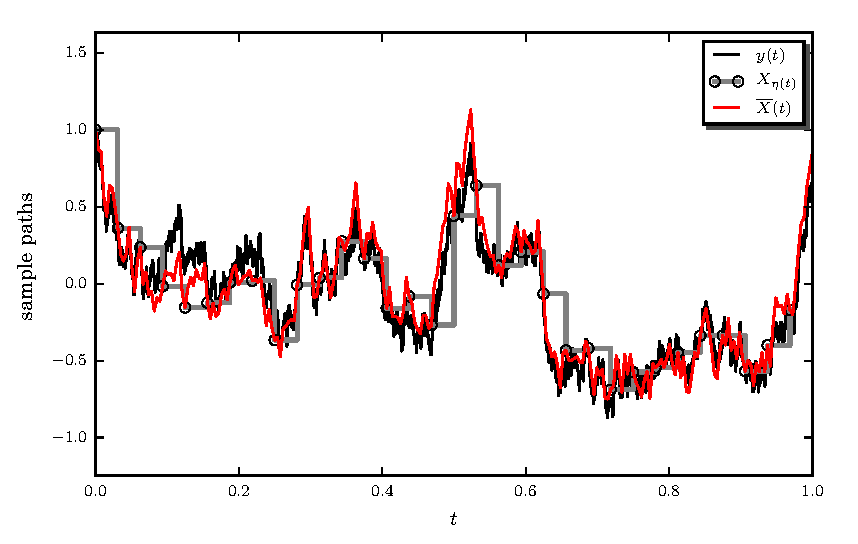
\includegraphics{papers/paperB/sections/ContinuousExtPy/ContinuousExtension.eps}
%	\caption{
%		The red line represents the continuous extension of the EM scheme. The continuous gray line is the $X_{\eta(t)}$ 
%		process defined in \eqref{eqn:EulerMaruyamaHigham}.
%	}
%	\label{fig:ContinuousExtension}
%\end{figure}

	Using the continuous extension \eqref{eqn:EMContinuousExtension} %or \eqref{eqn:EMIntegralContinuousExtension} 
and the uniform mean square norm, the authors work with a stronger version of the ms-error%, which is given by 
$$
	\EX{\sup_{0\leq t \leq t}|y(t)-\overline{X}(t)|^2}.
$$
%
So, in  order to prove the strong convergence of the EM method, the following assumptions are required.
\begin{assumption}\label{ass:HighamAssumption}
	For each $R>0$ there is a constant $C_R$, depending only on $R$, such that
	\begin{equation}\label{ass:LipschitzCondition}
		|f(x)-f(y)|^2 \vee |g(x)-g(y)|^2 \leq C_R|x-y|^2,
		\quad
		\forall x,y\in \R^d 
		\text{ with } |x|\vee |y|\leq R.
	\end{equation}
	And for some $p>2$, there is a constant $A$ such that
	\begin{equation}
		\EX{\sup_{0\leq t\leq T}|\overline{X}(t)|^p}
		\vee
		\EX{\sup_{0\leq t\leq T}|y(t)|^p} \leq A.
	\end{equation}
\end{assumption}
In \cite{Higham2002b}, the authors prove that the \Cref{ass:HighamAssumption} is sufficient to ensure strong 
convergence for the EM scheme, namely 
\begin{thm}[
	{\cite[Thm 2.2]{Higham2002b}}
	]\label{thm:HighamMaoStuart}
	Under \Cref{ass:HighamAssumption}, the EM scheme \eqref{eqn:EulerMaruyamaHigham} with continuous extension
	\eqref{eqn:EMContinuousExtension}
	%\eqref{eqn:EMIntegralContinuousExtension} 
	satisfies
	\begin{equation}
		\lim_{h\to 0}
		\EX{\sup_{0\leq t\leq T}|\overline{X}(t)-y(t)|^2}=0.
	\end{equation}
\end{thm}
	
	Applying this result, the authors prove the strong convergence of an implicit split-step variant of the EM, the
SSEM method. 
Their technique consist in proving each assertion of the following steps.
\begin{enumerate}[\bf{Step} 1:]
	\item
		\label{stp:EMCorrespondence}
		The SSEM for SDE \eqref{eqn:SDE1} is equivalent to the EM for the following conveniently SDE
		\begin{equation}\label{eqn:PerturbedHighamSDE}
			dx_h(t)= f_h(x_h(t))dt +g_h(x_h(t))dW(t).
		\end{equation}
	\item\label{stp:PerturbedSolution}
			The solution of the modified SDE \eqref{eqn:PerturbedHighamSDE} has bounded moments and it is 
			"close" to  $y$ the sense of the uniform mean square norm 
			$
				\EX{\sup_{0\leq t\leq T}|\cdot|^2}
			$.
	\item
	\label{stp:MethodBoundedMoments}
		Show that the SSEM method for the SDE \eqref{eqn:SDE1} has bounded moments.
	\item
		There is a continuous extension of the SSEM, $\overline{Z}(t)$, with bounded moments.
	\item
		Use the above steps and \Cref{thm:HighamMaoStuart} to conclude that
		\begin{equation}
			\lim_{h\to 0}
			\left\{
				\EX{\sup_{0\leq t\leq T}|x_h(t)-y(t)|^2}
			+
			\EX{\sup_{0\leq t\leq T}|\overline{Z}(t) -y_h(t)|^2}
			\right\}=0.
		\end{equation}
\end{enumerate}

	In the next section, using \Cref{thm:HighamMaoStuart} and this technique, we will prove the strong convergence of the 
\SM method \crefrange{eqn:SSLSM1}{eqn:SSLSM2}.
% We will 
%use the same technique as these authors, that is, we will show that:
%\begin{inparaenum}[(a)]
%	\item
%		the underlying method corresponds to the EM for a perturbed SDE and
%	\item
%		all moments of the approximation are bounded.
%\end{inparaenum}


\section{Strong Convergence of the Linear Steklov Method} 

	Here, we state and prove the main result of this chapter, the strong convergence of the \SM method
 \crefrange{eqn:SSLSM1}{eqn:SSLSM2} for the solution of SDE \eqref{eqn:SDE1}.
The main idea of the proof consist in applying the technique discussed in the previous section.
We begin establishing the underlying convergence theorem.
\begin{thm} %[Strong Convergence of the \SM method]
%\begin{restatable}[Strong Convergence of the \SM]{theorem}{StrongConvergence}
	\label{thm:StrongConvergenceLSMethod}
	Let \Cref{ass:OSLC} and \Cref{ass:ajBound} hold, consider the \SM method \crefrange{eqn:SSLSM1}{eqn:SSLSM2} for the 
	SDE	\labelcref{eqn:SDE1}.
	Then there is a continuous-time extension $\overline{Y}(t)$ of the \SM solution $\{Y_k\}$ for which 
	$\overline{Y}(t_k)=Y_k$ and
	\begin{equation*}
	\lim_{h \to 0}
	\EX{
		\sup_{0\leq t \leq T}
		|\overline{Y}(t) - y(t)|^2	
	}=0.
	\end{equation*} 
\end{thm}
%\end{restatable}
%Before to apply the HMS technique we will prove
To proof this result, we initiate with the first step of the HMS technique, that is, we will show that the \SM method
for SDE \eqref{eqn:SDE1} is equivalent to the EM scheme applied to the conveniently modified SDE
	\begin{equation} \label{eqn:SDEMod}
		dy_h(t)= \varphi_{f_h}(y_h(t))dt +g_h(y_h(t))dW(t),
		\qquad y_h(0)=y_0,  \qquad t\in [0,T].
	\end{equation}
We formalize this as a Corollary of \Cref{lem:PhiFhProp}.
%======================================================================================================================
%                                                 STEP 1                                                              %
%======================================================================================================================

\begin{corollary}\label{col:SSSMeEMmod}
	Let \Cref{ass:OSLC} and \Cref{ass:ajBound} holds, then the \SM method for SDE \eqref{eqn:SDE1} is 
	equivalent to the EM scheme applied to the modified SDE \eqref{eqn:SDEMod}.
\end{corollary}
\begin{pf}
	Using the functions $\varphi_{f_h}(\cdot)$ and $g_h(\cdot)$ defined in \eqref{eqn:FunctionshDefinition} of 
	\Cref{lem:PhiFhProp}, we 
	can rewrite the \SM method \Crefrange{eqn:SSLSM1}{eqn:SSLSM2} as 
	$$
		Y_{k+1} = Y_k + h \varphi_{f_h}(Y_k) + g_h(Y_k)\Delta W_k,
	$$
	which is the EM approximation for the modified SDE \eqref{eqn:SDEMod}. \qed
\end{pf}
%======================================================================================================================
%                                                 STEP 2                                                              %
%======================================================================================================================

	Now we proceed with the Step 2, that is,  we will prove that the solution  of the modified
SDE \eqref{eqn:SDEMod} has bounded moments and is close in uniform mean square norm to the solution of the SDE 
\eqref{eqn:SDE1}.
\begin{lem}\label{lem:BoundAndConvergenceOfyh}
	Let \Cref{ass:OSLC} and \Cref{ass:ajBound} holds. Then there is a constant $C=C(p,T)>0$ and a sufficiently small
	step size $h$, such that for all $p>2$
	\begin{equation}\label{eqn:yh-MomentBounds}
		\m\left[
			\sup_{0\leq t \leq T}
				|y_h(t)|^p
		\right]
		\leq
			C
		\left( 
			1+\m |y_0|^p
		\right).
	\end{equation}
	Moreover
	\begin{equation}\label{eqn:yh-convergence}
	\lim_{h \to 0}
	\m\left[
	\sup_{0\leq t \leq T}
	|y(t)-y_h(t)|^2
	\right]=0.
	\end{equation}
\end{lem}
\begin{pf}
	The bound \eqref{eqn:yh-MomentBounds} follows from inequality \eqref{eqn:h-MonotoneCondition} in
	\Cref{lem:PhiFhProp} and \Cref{thm:MaoCoercive}.
	On the other hand, to prove \eqref{eqn:yh-convergence} we will use the properties of 
	$\varphi_{f_h}$ and the Higham's stopping time technique employed in \cite[Thm 2.2]{Higham2002b}. 
	Note that by \Cref{lem:PhiFhProp} 
	\begin{align*}
		\varphi_{f_h}(x) 
			&= \Phi(h,a_j)(u) f^{(j)}(u) \1{E_j^c}(u) 
				+ f^{(j)}(u) \1{E_j}(u).
	\end{align*}
	Furthermore, by \Cref{ass:HypThmSingularities}  and since $f \in C^1(\R^d)$,   $\Phi(h,a_j)(\cdot)$ is bounded,
	hence, there is a positive constant $K_n$which depends only $n$ such that for each $j\in \{1,\dots, d\}$
	\begin{align*}	
		|\varphi_{f_h}^{(j)}(u) - f^{(j)}(u)|
		&\leq
			\1{E_j^c}(u)
			|f^{(j)}(u)|
			\left|
				\Phi(h,a_j)(u) - 1
			\right| \notag \\
		&\leq
			\1{E_j^c}(u)
			\left(
				C_h + 1
			\right)
			|f(u)|	 \notag \\
		&\leq
		\1{E_j^c}(u) K_n(C_h+1), \quad \forall u \in \R^d, \quad |u|\leq n,  \quad \forall j\in \{1,\dots, d\}.
	\end{align*}
	Moreover, we know by the proof of \Cref{lem:PhiFhProp} that
	\begin{equation*}
	 \lim_{
	 	\substack{
		 	h\to 0 \\
		 	u\in E_j^c	
	 	}
	 }
	 \Phi(h,a_j)(u) = 1.	 	
	\end{equation*}
	Also, we note that for each $j \in \{1, \dots , d\}$
	\begin{equation*}
	\lim_{h \to 0} F_h^{(j)}(u)
		=
		\lim_{h \to 0}
			e^{ha_j(u)} u^{(j)} + 
		\lim_{h \to 0}
			\left(
				\frac{e^{ha_j(u)}-1}{a_j(u)}
				\1{E_j^c}(u)
				+h \1{E_j}(u)
			\right)
			b_j(u^{(j)}) 
		= u^{(j)},
	\end{equation*}
	hence
	$%\begin{equation*}
		\displaystyle
		\lim_{h\to 0} F_h(u)=u.
	$ %\end{equation*}
	Consequently, given $n>0$ there is  a function $K_n(\cdot):(0,\infty)\to (0,\infty)$, such that
	$K_n(h)\to 0$ when $h \to 0$ and
	\begin{equation}\label{eqn:PhihGhKRhBound}
		|\varphi_{f_h}(u)-f(u)|^2 \vee |g_h(u)-g(u)|^2
		\leq K_n(h) \qquad \forall u\in \R^d, \quad |u| \leq n.
	\end{equation}
	Now, using that both $f$, $g$ are $C^{1}$, there is  a constant $H_n>0$ such that
	\begin{equation}\label{eqn:f-gHRBound}
		|f(u)-f(v)|^2 \vee |g(u)-g(v)|^2
		\leq H_n |u-v|^2\qquad \forall u,v \in \R^d, |u|\vee |v| \leq n.
	\end{equation}
	
		On the other hand, by \Cref{lem:MomentBound} and inequality \eqref{eqn:yh-MomentBounds} we obtain
	\begin{equation*}
		\m\left[
			\sup_{0\leq t \leq T}
				|y(t)|^p
		\right]
		\vee
		\m\left[
			\sup_{0\leq t \leq T}
				|y_h(t)|^p
		\right]
		\leq
		K := C
		\left( 
			1+\m |y_0|^p
		\right).
	\end{equation*}
	Now, we define the stopping times
	\begin{equation}\label{eqn:StoppingTimes}
		\tau_n := 
			\inf\{
				t\geq 0: |y(t)|\geq n
			\},
		\qquad
		\rho_n := 
			\inf\{
				t\geq 0: |y_h(t)|\geq n
			\},
		\qquad
		\theta_n:=
			\tau_n \wedge \rho_n,
	\end{equation}
	and the difference function
	\begin{equation*}
		e_h(t):= y(t) - y_h(t).
	\end{equation*}
	From the Young's inequality \eqref{eqn:YoungsInequality}, we deduce that for any $\delta>0$ 
	\begin{align}
		\m\left[
			\sup_{0\leq t\leq T}
			|e_h(t)|^2
		\right]
		&=
			\m\left[
				\sup_{0\leq t\leq T}
				|e_h(t)|^2
				\1{\tau_n>T,\rho_n>T}
			\right]
			+
			\EX{
				\sup_{0\leq t\leq T}
				|e_h(t)|^2
				\1{\tau_n \leq T \text{ or } \rho_n \leq T}
			}\notag\\
		&\leq
			\EX{
				\sup_{0\leq t\leq T}
				|e_h(t\wedge \theta_n)|^2
				\1{\theta_n \geq T}
			}
			+\frac{2\delta}{p}
			\EX{
				\sup_{0\leq t\leq T}
				|e_h(t)|^p 
			}\notag \\
		&+
			\frac{1-2/p}{\delta^{2/(p-2)}}
			\Prob{\tau_n \leq T \text{ or } \rho_n \leq T}.
	\label{eqn:AfterYoungIneq}
	\end{align}
	We proceed to bound each term on the right-hand side of inequality \eqref{eqn:AfterYoungIneq}.
	By \Cref{lem:MomentBound}, $y(t)$ has bounded moments, hence 
	there is a positive constant $A$ such that
	\begin{equation}\label{eqn:BoundProbTauR}
		\Prob{\tau_n\leq T}
		=
			\EX{\1{\tau_n<T}\frac{|y(\tau_n)|^p}{n^p}}
		\leq
			\frac{1}{n^p}\EX{\sup_{0\leq t\leq T}|y(t)|^p} \leq \frac{A}{n^p},
			\qquad \text{for } p\geq 2.
	\end{equation}
	The same conclusion can be drawn for $\rho_n$, then
	\begin{equation} \label{eqn:BoundProbTauRorRhoR}
		\Prob{\tau_n \leq T \text{ or } \rho_n \leq T}
		\leq
			\Prob{\tau_n\leq T}+\Prob{\rho_n\leq T}
		\leq
		\frac{2A}{n^p}.
	\end{equation}
	Now, using the inequality \eqref{eqn:SingleHolder} and \Cref{lem:MomentBound} we have
	\begin{equation} \label{eqn:ehMomentBound}
		\EX{
			\sup_{0\leq t \leq T}
			|e_h(t)|^p
		}
		\leq
		2^{p-1}
		\EX{
			\sup_{0 \leq t \leq T}
			\left(
			|y(t)|^p + |y_h(t)|^p
			\right)
		}
		\leq 2^pA.
	\end{equation}
%
	So, combining the bound \eqref{eqn:BoundProbTauRorRhoR} with \eqref{eqn:ehMomentBound}
	in inequality \eqref{eqn:AfterYoungIneq} we obtain
	\begin{align}
		\EX{
			\sup_{0\leq t \leq T}
			|e_h(t)|^2
		}
		&\leq
			\EX{
				\sup_{0\leq t\leq T}
				|e_h(t\wedge \theta_n)|^2
				\1{\theta_n \geq T}
			}
	%\notag \\
			+\frac{2^{p+1}\delta A}{p}
			+\frac{2(p-2)A}{p\delta^{2/(p-2)}n^p}. \label{eqn:TermToBound}
	\end{align}
	Next, we show that the first term of \eqref{eqn:TermToBound} is bounded. Adding conveniently terms yields
	\begin{align*}
		e_h(t\wedge\theta_n) 
			&=
			\int_{0}^{t\wedge\theta_n}
			\left[
				f(y(s)) - f(y_h(s))+f(y_h(s))
				-\varphi_{f_h}(y_h(s))
			\right]ds \notag \\
			&+
			\int_{0}^{t\wedge\theta_n}
			\left[
				g(y(s)) - g(y_h(s))+g(y_h(s))
				-g_h(y_h(s))
			\right]dW(s).
	\end{align*}
	Using the bounds \eqref{eqn:PhihGhKRhBound} and \eqref{eqn:f-gHRBound}, the Cauchy-Schwarz, and
	Doob martingale inequalities, we get
	\begin{align*}
		\EX{\sup_{0\leq t \leq \tau}|e_h(t\wedge\theta_n)|^2}
		&\leq 
		4H_n(T+4)
		\int_{0}^{\tau}
			\EX{\sup_{0\leq t \leq \tau}|e_h(t\wedge\theta_n)|^2} ds 
		+
		4T(T+4)K_n(h).\notag
	\end{align*}
	The Gronwall inequality now yields
	\begin{align*}
		\EX{\sup_{0\leq t \leq T}|e_h(t\wedge\theta_R)|^2}
		&\leq
			4T(T+4)K_n(h)\exp(4H_n(T+4)T). %\notag \\
	%+
	%\frac{2^{p+1}\delta A}{p}
	%+
	%\frac{(p-2)2A}{p\delta^{2/(p-2)}R^p}.
	\end{align*}
	Hence, given $\epsilon>0$ for any $\delta>0$ such that
	$
		2^{p+1}\delta A/p< \epsilon/3,
	$
		we can take $n>0$ verifying
	$
		(p-2)2A/(p\delta^{2/(p-2)}n^p)<\epsilon/3.
	$
	Moreover, we can take $h$ sufficiently small such that
	$
		4T(T+4)K_n(h)\exp(4H_n(T+4)T) < \epsilon/3. 
	$
	It follows immediately that
	$$
		\EX{\sup_{0\leq t \leq T}|e_h(t)|^2}
		<
			\epsilon/3
			+\epsilon/3
			+\epsilon/3
		=\epsilon,
	$$ which is the desired conclusion.\qed
\end{pf}
%======================================================================================================================
%                                                 STEP 3                                                              %
%======================================================================================================================

	Next, we proceed with Step 3, in which we establish that \SM method has bounded moments.
\begin{lem}\label{lem:SSSMMomentBounds}
	Let \Cref{ass:OSLC}, \Cref{ass:ajBound}  and \Cref{ass:HypThmSingularities} holds. Then for each $p\geq 2$ there is 
	a universal positive constant 
	$C=C(p,T)$ 
	such that for the \SM method
	\begin{equation*}
		\m\left[
		\sup_{kh \in [0,T]}
		|Y_k|^{2p}
		\right]\leq C.
	\end{equation*}
\end{lem}
\begin{pf}
	Using the split formulation of the \SM scheme \crefrange{eqn:SSLSM1}{eqn:SSLSM2} we get
	\begin{dmath}[label=leqn:Yn2Bound]
		|Y_k^{\star}|^{2}
		\leq
			|A^{(1)}(h,Y_k)|^2 |Y_k|^2  
			+ 2 \innerprod{A^{(1)}(h,Y_k)Y_k}{A^{(2)}(h,Y_k) Y_k b(Y_k)}
			+|A^{(2)}(h,Y_k)|^2 |b(Y_k)|^2.
	\end{dmath}
	Then, applying the Cauchy-Schwartz inequality and \Cref{ass:ajBound} we arrive at
	\begin{dmath*}[label=leqn:Yn2Bound]
		|Y_k^{\star}|^{2}
		\leq
		|A^{(1)}(h,Y_k)|^2 |Y_k|^2  
		+ 2 \sqrt{L_b} d|A^{(1)}(h,Y_k)||A^{(2)}(h,Y_k)||Y_k|(1+|Y_k|)
		+L_b|A^{(2)}(h,Y_k)|^2 (1+|(Y_k)|^2).
	\end{dmath*}
	Using \eqref{ass:ajBound} we see that
	\begin{dmath}[label=eqn:A1Bound]
		|A^{(1)}(h,Y_k)|^2 
		=
			\left|
				\diag
				\left(
					e^{ha_1(Y_k)}, \dots, e^{ha_d(Y_k)} 
				\right)
			\right|^2
		\leq
		 \underbrace{d \exp( 2 T L_a)}_{:= L_{A^{(1)}}}.		
	\end{dmath}
	In similar way, we deduce from the bound \eqref{eqn:PhiBound} that
	\begin{align}
		|A^{(2)}(h,Y_k)|^2 
		&=
		\left|
			h 
			\diag
			\left(
				\1{E_1}(Y_k)
				+\1{E_1^c}(Y_k)\Phi(h,a_1)(Y_k), 
				\dots,
				\1{E_d}(Y_k)
				+\1{E_d^c}(Y_k) \Phi(h,a_d)(Y_k)
			\right)
		\right|^2 \notag \\
		%
		&\leq
		\sum_{j=1}^{d}
		\left(
			\1{E_j^c}
			|h\Phi(h,a_1)(Y_k)|^2
			+ h^2
		\right)
		\leq
		\underbrace{
			2\exp(2 L_a  T)
				\sum_{j=1}^d
				\frac{1}{a_j^*} + d T^2.			
		}_{:=L_{A^{(2)}}}
		\label{eqn:A2Bound}
	\end{align}
	Combining \eqref{eqn:bjLinearGrowthCondition} of \Cref{ass:ajBound} with bounds \eqref{eqn:A1Bound}
	and \eqref{eqn:A2Bound} yields
	\begin{align*}
		|Y_k^{\star}|^2
		&\leq
			L_{A^{(1)}} |Y_k|^2
			+ 2 d \sqrt{L_{A^{(1)}} L_{A^{(2)}} L_b }|Y_k|(1+|Y_k|)
			+L_{A^{(2)}} L_b (1+|Y_k|^2).
	\end{align*}
	So, taking $\widetilde{C}\geq L_{A^{(1)}}+ 2 d \sqrt{L_{A^{(1)}} L_{A^{(2)}} L_b} + L_{A^{(2)}} L_b$ we can assert 
	that
	\begin{equation}\label{eqn:YkStarBound}
		|Y^{\star}_k|^2
			\leq 
				\widetilde{C}(3|Y_k|^2+|Y_k| + 1) 
			\leq 
				6\widetilde{C}\left(
					|Y_k|^2+1
				\right)
			\leq C(1+|Y_k|^2).
	\end{equation} 
	Then, applying bound \eqref{eqn:YkStarBound} in \cref{eqn:SSLSM2} we arrive at
	\begin{equation*}
		|Y_{k+1}|^2
		\leq
			C \left(
				|Y_k|^2 + 1
			\right)
			+ 2\innerprod{Y^{\star}_k}{g(Y^{\star}_k) \Delta W_k}
			+ \left|g(Y^{\star}_k) \Delta W_k \right|^2
	\end{equation*}
	Now, we choose two integers $N,M$ such that $Nh\leq Mh \leq T$. So, adding backwards we get
	\begin{align*}
		|Y_N|^2
			&\leq
			S_N\left(
				\sum_{j=0}^{N-1}
					(1+|Y_j|^2)
				+
				2\sum_{j=0}^{N-1}
					\innerprod{Y_j^{\star}}{g(Y_j^{\star}) \Delta W_j}
				+
				\sum_{j=0}^{N-1}
					\left|
						g(Y_j^{\star}) \Delta W_j
					\right|^2
			\right)\\
			S_N
				&:=
				\sum_{j=0}^{N-1}
					C^{N-j} 			
	\end{align*}

	Raising both sides to the power $p$ and using the standard inequality \eqref{eqn:SingleHolder} we obtain
	\begin{align}\label{eqn:RelationToBound}
		|Y_N|^{2p}	
			&\leq
				6^{p} S_N^p
				\left(
					N^{p-1}
						\sum_{j=0}^{N-1}
						(1+|Y_j|^{2p})	
					+
					\left|
						\sum_{j=0}^{N-1}
						\innerprod{Y_j^{\star}}{g(Y_j^{\star}) \Delta W_j}
					\right|^p
					+
					N^{p-1}
					\sum_{j=0}^{N-1}
						\left|
							g(Y_j^{\star}) \Delta W_j
						\right|^{2 p}				
				\right)
	\end{align}
	Now we will show that the second and third terms of the inequality \eqref{eqn:RelationToBound} are bounded.
	We denote by $C=C(p,T)$ an generic positive constant that not depends on  the step size $h$ and whose
	value may changes between occurrences.
	Next, using the Bunkholder-Davis-Gundy inequality,
	%\cite[Thm 7.3 pg. 40]{XMao461}
	\eqref{thm:BDG}
	we see that
	\begin{align}\label{eqn:BoundSecondTerm}
		\m
		\left[
			\sup_{0\leq N \leq M}
			\left|
				%\exp(2hpNL)
				\sum_{j=0}^{N-1}
					\innerprod{Y_j^{\star}}{g(Y_j^{\star})\Delta W_j}
			\right|^{p}
		\right]
		&\leq
			C\m
			\left[
				\sum_{j=0}^{N-1}
					|Y_j^{\star}|^2
					|g(Y_j^{\star})|^2
					h
			\right]^{p/2}
			\notag\\
		&\leq
			C h^{p/2}M^{p/2-1}
			\m
				\sum_{j=0}^{M-1}
					|Y_j^{\star}|^p (\alpha +\beta |Y_j^{\star}|^2)^{p/2}
			\notag\\
		&\leq
			2^{p/2-1}C T^{p/2-1} h  
			\m
			\sum_{j=0}^{M-1}
				(\alpha^{p/2}|Y_j^{\star}|^p +\beta^{p/2} |Y_j^{\star}|^{2p})
			\notag\\
		&\leq
			C h
			\m
			\sum_{j=0}^{M-1}
				(1+2|Y_j^{\star}|^p + |Y_j^{\star}|^{2p})
			\notag\\
		&\leq
			C h 
			\sum_{j=0}^{M-1}
			\left[
				1+\m|Y_j^{\star}|^{2p}
			\right]
			\notag\\
		&\leq
			C 
			+ 
			C h 
			\sum_{j=0}^{M-1}
				\m|Y_j|^{2p}	
			.
	\end{align}
	%
	Now, note that 
	\begin{equation}\label{eqn:SupOfSum}
		\EX{
			\sup_{0\leq N\leq M}
				\sum_{j=0}^{N-1}
				|Y_j|^{2p}
		}
		=
		\sum_{j=0}^{M-1}
			\m|Y_j|^{2p}.
	\end{equation}
	Hence, using Cauchy-Schwartz inequality, the monotone condition 
	\eqref{ass:MonotoneCondition}, bound \eqref{eqn:YkStarBound}
	and the standard inequality \eqref{eqn:SingleHolder}, we obtain
	\begin{align}
	\m\left[
		\sup_{0\leq N \leq M}
			\sum_{j=0}^{N-1}
			\left|
				g(Y_j^{\star})\Delta W_j
			\right|^{2p}	
		\right]
		&=
			\m
				\sum_{j=0}^{M-1}
					\left|
						g(Y_j^{\star})\Delta W_j
					\right|^{2p}
			\notag\\
		&\leq	
			\sum_{j=0}^{M-1}
				\m
					\left|
						g(Y_j^{\star})
					\right|^{2p}
				\m
					\left|
						\Delta W_j
					\right|^{2p}
			\notag \\
		&\leq
			C h^p
			\sum_{j=0}^{M-1}
			\m
				\left[
					\alpha +\beta|Y^{\star}_j|^2
				\right]^p
			\notag\\
	%
		&\leq
			Ch^p
			\sum_{j=0}^{M-1}
			\m
				\left[
					\alpha ^p +\beta^p |Y^{\star}_j|^{2p}
				\right]
			\notag\\
		&\leq
		Ch^{p-1}
		+
		Ch^p \sum_{j=0}^{M-1}
			\m|Y_j|^{2p} \label{eqn:BoundThirdTerm}.
	\end{align}
	Thus, combining the bounds \eqref{eqn:BoundSecondTerm} and \eqref{eqn:BoundThirdTerm} with the inequality 
	\eqref{eqn:RelationToBound}, we can assert that
	\begin{align}
		\EX{
			\sup_{0\leq N \leq M}
					|Y_N|^{2p} 
		}
		&\leq
			C(M,T) + C(M,T)(1+h)
			\sum_{j=0}^{M-1}
				\m|Y_j|^{2p}  
			\notag \\
		&\leq	
			C +C(1+h) 
			\sum_{j=0}^{M-1}
				\EX{
					\sup_{0\leq N \leq j}
					|Y_N|^{2p}
				}	
		.
	\end{align}
	Finally, using the discrete-type Gronwall inequality \eqref{thm:DiscreteGronwall}, we conclude that
	\begin{align*}
		\EX{
			\sup_{0\leq N \leq M}
			|Y_N|^{2p} 
		}	
		&\leq
			C\exp(C(1+h)M) 
		\leq 
		C \exp(C(1+T))<C,
	\end{align*}
	since the constant C does not depend on $h$, the proof is complete. \qed
\end{pf}
%======================================================================================================================
%                                                 STEP 4                                                              %
%======================================================================================================================
	
	As the \SM scheme has bounded moments, we now proceed whit Step 4, so we will obtain a convenient 
continuous extension of the \SM method with bounded moments. 
Let $\{Y_k\}$ denote the \SM solution of SDE \eqref{eqn:SDE1}.
By \Cref{col:SSSMeEMmod}, it is feasible to constructs a continuous extension for the \SM approximation, from the 
time continuous extension of the EM \eqref{eqn:EMContinuousExtension}.
Moreover, we would expect that the moments of this new extension remains bounded.
\begin{corollary}\label{col:ContinuousExtBoundedMoments}
	Let \Cref{ass:OSLC}, \Cref{ass:ajBound}  and \Cref{ass:HypThmSingularities} holds and suppose  $0<h<1$ and $p\geq 
	2$. Then there is a continuous extension $\overline{Y}(t)$ of $\{Y_k\}$  and a positive constant $C=C(T,p)$ such 
	that
	\begin{equation*}
		\EX{\sup_{0\leq t \leq T} |\overline{Y}(t)|^{2p} }
		\leq C.
	\end{equation*}
\end{corollary}
	\begin{pf}
		We take $t=s+t_k$ in $ [0,T]$, $\Delta W_k(s):= W(t_k+s)- W(t_k)$ and $0\leq s <h$.
		Then we define 
		\begin{equation}\label{eqn:SSLSContinuousExtension}
			\overline{Y}(t_k+s):= Y_k + s \varphi_{f_h}(Y_k) + g_h(Y_k)\Delta W_k(s),
		\end{equation}
		as a continuous extension of the \SM scheme. We proceed to show that $\overline{Y}(t)$ has bounded moments.
		By \Cref{lem:PhiFhProp}, we have $Y_k^{\star}= Y_k + h \varphi_{f_h}(Y_k)$. 
		Then for $\gamma = s/h$, it follows that
		\begin{align*}
			Y_k + s \varphi_{f_h}(Y_k)
			&= 
			\gamma (Y_k + h \varphi_{f_h}(Y_k)) +(1-\gamma)Y_k\\
			&=
			\gamma Y_k^{\star} + (1-\gamma)Y_k.
		\end{align*}
		Hence, we can rewrite the continuous extension \eqref{eqn:SSLSContinuousExtension} as
		\begin{align}
			\overline{Y}(t) &=
			\gamma Y^{\star}_k + (1-\gamma) Y_k +g_h(Y_k) \Delta W_k(s). %\label{eqn:SSLSMConExt}
			\notag
		%t&=t_k+s,  \qquad  \gamma = s/h\qquad s\in {[0,h)]}.\notag
		\end{align}
		%
		Combining this relation with  the inequalities \eqref{eqn:YkStarBound} and \eqref{eqn:SingleHolder}, we arrive 
		at
		\begin{align}
			|\overline{Y}(t_k+s) |^2 
			&\leq
				3\left[
					\gamma C
					+
					\left(
						\gamma C +1 - \gamma
					\right)
					|Y_k|^2
					+
					|g_h(Y_k)\Delta W_k(s)|^2
			\right] \notag\\
		&\leq
			C
			+
			C
			\left(
				|Y_k|^2 + |g_h(Y_k)\Delta W_k(s)|^2
			\right).
		\notag
		\end{align}
	\end{pf}
	Thus, 
	\begin{align}
		\sup_{0\leq t\leq T} |\overline{Y}(t)|^{2p}
		&\leq
			\sup_{0\leq kh\leq T}
			\left[
				\sup_{0\leq s\leq h}
					|\overline{Y}(t_k+s)|^{2p} 
			\right] 
		\notag\\
		&\leq
			\sup_{0\leq kh\leq T} 
			\left[
				\sup_{0\leq s\leq h}
					C 
					\left(
						1 + |Y_k|^{2p} + |g_h(Y_k)\Delta W_k(s)|^{2p}
					\right)
			\right],
		\label{eqn:BeforeDoob}
	\end{align}
	for $t\in [0,T]$.
	%
	Now taking a non negative integer $0 \leq k \leq N$ such that $0\leq Nh \leq T$. From the bond 
	\eqref{eqn:BeforeDoob}, we get
	\begin{align}
		\sup_{0\leq t\leq T} |\overline{Y}(t)|^{2p}
		&\leq 
			C
			\left(
				1
				+
				\sup_{0\leq kh\leq T} 
					|Y_k|^{2p}
					+
					\sup_{0\leq s\leq h}
						\sum_{j=0}^N
							|g_h(Y_j)\Delta W_j(s)|^{2p}
			\right) \label{eqn:SumDiffusion}.
	\end{align}
	So, using the Doob's Martingale inequality \eqref{eqn:DoobMartingaleInequality},
	\Cref{lem:SSSMMomentBounds} and that $g_h$ is a locally 
	Lipschitz function, we can bound each term of the inequality \eqref{eqn:SumDiffusion},  as follows
	\begin{align}
		\EX{
			\sup_{0 \leq s \leq h} |g(Y_j) \Delta W_j(s)|^{2p}
		}
		&\leq
			\left(
				\frac{2p}{2p-1}
			\right)^{2p}
			\m|g_h(Y_j)\Delta W_j(h)|^{2p}
			\notag
			\\
		&\leq
			C \m |g_h(Y_j)|^{2p} \m |\Delta W_j(h)|^{2p} \notag\\
		&\leq
			C h^p
			\left(
				1 + \m|Y_j|^{2p}
			\right) \notag \\
		& \leq C h, \label{eqn:BeforeConclusion}
	\end{align}
	for each $j \in \{0,\dots, N\}$.
	Since $Nh\leq T$, combining the bounds \eqref{eqn:SumDiffusion} and \eqref{eqn:BeforeConclusion} we 
	get the desired conclusion. \qed
%======================================================================================================================
%                                                 STEP 5                                                              %
%======================================================================================================================

	Once we have carried out all the previous steps, we can prove the \Cref{thm:StrongConvergenceLSMethod} by Step 5.%
%We are now in a position to execute the \textbf{Step 5}.
\begin{pf}[of Theorem \ref{thm:StrongConvergenceLSMethod}]
	First,  note that by inequality \eqref{eqn:SingleHolder}, we have
	\begin{align}\label{eqn:AfterTriangle}
		\EX{\sup_{0\leq t \leq T}|\overline{Y}(t) - y(t)|^2}
		&\leq
		2\EX{
			\sup_{0\leq t \leq T}
			|\overline{Y}(t) - y_h(t)|^2
		}
		+
		2\EX{
			\sup_{0\leq t \leq T}
			|y_h(t) - y(t)|^2
		}.
	\end{align}
	Using \Cref{lem:BoundAndConvergenceOfyh}, which was established in the Step 2, yields
	\begin{equation}\label{eqn:SeconTermZeroLim}
		\lim_{h\to 0}
		\EX{
			\sup_{0\leq t \leq T}
			|y_h(t) - y(t)|^2
		} = 0.
	\end{equation}
	
		It remains to prove that the first term of the right hand side in inequality \eqref{eqn:AfterTriangle} 
		decreases to zero
	when $h$ tends to zero. Recalling that:
	\begin{enumerate}[i)]
	%\begin{inparaenum}[\itshape i\upshape)]
		\item 
			By \Cref{lem:BoundAndConvergenceOfyh}, the solution of the modified SDE \eqref{eqn:SDEMod}, $y_h$, has
			$p$-bounded moments ($p\geq 2$).
		\item
			By \Cref{col:ContinuousExtBoundedMoments}, the \SM continuous extension for the SDE \eqref{eqn:SDE1},
			$\overline{Y}(t)$, has bounded moments and it is equivalent to the EM extension for the modified SDE 
			\eqref{eqn:SDEMod}.
		%\end{inparaenum}
	\end{enumerate}
	Hence, we can apply 
	%\cite[Thm. 2.2]{Higham2002b} 
	\Cref{thm:HighamMaoStuart} to conclude that
\begin{equation}\label{eqn:FirstTermZeroLim}
	\lim_{h\to 0}
	\EX{
		\sup_{0\leq t \leq T}
		|\overline{Y}(t) - y_h(t)|^2
	} = 0.
\end{equation}
	Finally, combining the limits \eqref{eqn:SeconTermZeroLim} and \eqref{eqn:FirstTermZeroLim} with 
	inequality \eqref{eqn:AfterTriangle} gives
\begin{align*}
	%0\leq 
	\lim_{h \to 0}
	\EX{
		\sup_{0\leq t \leq T}
		|\overline{Y}(t) - y(t)|^2
	}
	\leq
	&
	2\lim_{h\to 0}
	\EX{
		\sup_{0\leq t \leq T}
		|\overline{Y}(t) - y_h(t)|^2
	}
	\\
	&
	+
	2\lim_{h\to 0}
	\EX{
		\sup_{0\leq t \leq T}
		|y_h(t) - y(t)|^2
	} = 0,
\end{align*}
which proves the theorem. \qed
\end{pf}

	\pagebreak
	\section*{\refname}
	\begin{thebibliography}{17}
\providecommand{\natexlab}[1]{#1}
\providecommand{\url}[1]{\texttt{#1}}
\expandafter\ifx\csname urlstyle\endcsname\relax
  \providecommand{\doi}[1]{doi: #1}\else
  \providecommand{\doi}{doi: \begingroup \urlstyle{rm}\Url}\fi

\bibitem[Appleby and Kelly(2010)]{Appleby2010}
J.~Appleby and C.~Kelly.
\newblock On the local dynamics of polynomial difference equations with fading
  stochastic perturbations.
\newblock \emph{Dynamics of Continuous, Discrete and Impulsive Systems}, pages
  401--430, 2010.
\newblock URL \url{http://strathprints.strath.ac.uk/id/eprint/29102
  http://strathprints.strath.ac.uk/41130/1/Colombo\_C\_et\_al\_Pure\_Stabilisation\_of\_the\_hyperbolic\_equilibrium\_of\_high\_area\_to\_mass\_spacecraft\_Oct\_2012.pdf
  http://strathprints.strath.ac.uk/29102/}.

\bibitem[Appleby et~al.(2008)Appleby, Mao, and Rodkina]{Appleby2008}
J.~Appleby, X.~Mao, and A.~Rodkina.
\newblock Stabilization and destabilization of nonlinear differential equations
  by noise.
\newblock \emph{IEEE Transactions on Automatic Control}, 53\penalty0
  (3):\penalty0 683--691, 2008.
\newblock ISSN 00189286.
\newblock \doi{10.1109/TAC.2008.919255}.

\bibitem[Beyn et~al.(2010)Beyn, Isaak, and Kruse]{Beyn2010}
Wolf-j\"{u}rgen Beyn, Elena Isaak, and Raphael Kruse.
\newblock Stochastic c-stability and b-consistency of explicit and implicit
  euler-type schemes.
\newblock pages 1--29, 2010.

\bibitem[D\'{\i}az-Infante and Jerez(2015)]{Diaz-Infante2015}
Sa\'{u}l D\'{\i}az-Infante and Silvia Jerez.
\newblock Convergence and asymptotic stability of the explicit steklov method
  for stochastic differential equations.
\newblock \emph{Journal of Computational and Applied Mathematics}, pages 1--12,
  2015.
\newblock ISSN 03770427.
\newblock \doi{10.1016/j.cam.2015.01.016}.
\newblock URL
  \url{http://linkinghub.elsevier.com/retrieve/pii/S037704271500028X}.

\bibitem[Fine(1966)]{FineAIandKass1966}
Kass~S. Fine, A.~I.
\newblock Indeterminate forms for multi-place functions.
\newblock \emph{Annales Polonici Mathematici}, 18\penalty0 (1):\penalty0
  59--64, 0 1966.

\bibitem[Guo et~al.(2014)Guo, Li, and Zhu]{Guo2014}
Qian Guo, Hongqun Li, and Ying Zhu.
\newblock The improved split-step $\theta$ methods for stochastic differential
  equation.
\newblock \emph{Mathematical Methods in the Applied Sciences}, 37\penalty0
  (August 2013):\penalty0 2245--2256, 2014.
\newblock ISSN 01704214.
\newblock \doi{10.1002/mma.2972}.
\newblock URL \url{http://doi.wiley.com/10.1002/mma.2972}.

\bibitem[Higham et~al.(2002)Higham, Mao, and Stuart]{Higham2002b}
Desmond~J Higham, Xuerong Mao, and Andrew~M Stuart.
\newblock Strong convergence of euler-type methods for nonlinear stochastic
  differential equations.
\newblock \emph{SIAM Journal on Numerical Analysis}, 40\penalty0 (3):\penalty0
  1041--1063, January 2002.
\newblock ISSN 0036-1429.
\newblock \doi{10.1137/S0036142901389530}.
\newblock URL \url{http://epubs.siam.org/doi/abs/10.1137/S0036142901389530}.

\bibitem[Hutzenthaler et~al.(2010)Hutzenthaler, Jentzen, and
  Kloeden]{Hutzenthaler2010}
M.~Hutzenthaler, A.~Jentzen, and P.~E. Kloeden.
\newblock Strong and weak divergence in finite time of euler's method for
  stochastic differential equations with non-globally lipschitz continuous
  coefficients.
\newblock \emph{Proceedings of the Royal Society A: Mathematical, Physical and
  Engineering Sciences}, 467\penalty0 (2130):\penalty0 1563--1576, December
  2010.
\newblock ISSN 1364-5021.
\newblock \doi{10.1098/rspa.2010.0348}.
\newblock URL
  \url{http://rspa.royalsocietypublishing.org/cgi/doi/10.1098/rspa.2010.0348}.

\bibitem[Hutzenthaler and Jentzen(2015)]{Hutzenthaler2015}
Martin Hutzenthaler and Arnulf Jentzen.
\newblock Numerical approximations of stochastic differential equations with
  non-globally lipschitz continuous coefficients.
\newblock \emph{Memoirs of the American Mathematical Society}, 236\penalty0
  (1112), July 2015.
\newblock ISSN 1947-6221.
\newblock \doi{http://dx.doi.org/10.1090/memo/1112}.
\newblock URL \url{http://www.ams.org/}.

\bibitem[Hutzenthaler et~al.(2012)Hutzenthaler, Jentzen, and
  Kloeden]{Hutzenthaler2012a}
Martin Hutzenthaler, Arnulf Jentzen, and Peter~E. Kloeden.
\newblock Strong convergence of an explicit numerical method for sdes with
  nonglobally lipschitz continuous coefficients.
\newblock \emph{The Annals of Applied Probability}, 22\penalty0 (4):\penalty0
  1611--1641, August 2012.
\newblock ISSN 1050-5164.
\newblock \doi{10.1214/11-AAP803}.
\newblock URL \url{http://projecteuclid.org/euclid.aoap/1344614205}.

\bibitem[Lamba et~al.(2007)Lamba, Mattingly, and Stuart]{Lamba2007}
H.~Lamba, J.~C. Mattingly, and a.~M. Stuart.
\newblock An adaptive euler-maruyama scheme for sdes: Convergence and
  stability.
\newblock \emph{IMA Journal of Numerical Analysis}, 27:\penalty0 479--506,
  2007.
\newblock ISSN 02724979.
\newblock \doi{10.1093/imanum/drl032}.

\bibitem[Lawlor(2012)]{Lawlor2012}
Gary~R Lawlor.
\newblock A l'hospital's rule for multivariable functions.
\newblock \emph{arXiv preprint arXiv:1209.0363}, 2012.

\bibitem[Liptser and Shiryayev(1989)]{Liptser1989}
Robert Liptser and A.~N. Shiryayev.
\newblock \emph{Theory of Martingales}.
\newblock Springer, Oct 1989.
\newblock ISBN 978-94-010-7600-5.

\bibitem[Mao(2007)]{Mao2007}
X~Mao.
\newblock \emph{Stochastic Differential Equations and Application}.
\newblock Horwood Pub., Dec 2007.
\newblock ISBN 978-19-0427-534-3.

\bibitem[Mao and Szpruch(2013)]{Mao2013}
Xuerong Mao and Lukasz Szpruch.
\newblock Strong convergence and stability of implicit numerical methods for
  stochastic differential equations with non-globally lipschitz continuous
  coefficients.
\newblock \emph{Journal of Computational and Applied Mathematics},
  238:\penalty0 14--28, January 2013.
\newblock ISSN 03770427.
\newblock \doi{10.1016/j.cam.2012.08.015}.
\newblock URL
  \url{http://linkinghub.elsevier.com/retrieve/pii/S0377042712003378
  http://strathprints.strath.ac.uk/13892/}.

\bibitem[Matus et~al.(2005)Matus, Irkhin, and
  Lapinska-Chrzczonowicz]{Matus2005}
P~Matus, U.~Irkhin, and M.~Lapinska-Chrzczonowicz.
\newblock Exact difference schemes for time-dependent problems.
\newblock \emph{Computational Methods in Applied Mathematics}, 5\penalty0
  (4):\penalty0 422--448, 2005.
\newblock ISSN 1609-4840.
\newblock \doi{10.2478/cmam-2005-0020}.
\newblock URL
  \url{http://old.cmam.info/issues/?Vol=5&Num=4&ItID=133&Type=pdf&Aid=133
  http://www.degruyter.com/view/j/cmam.2005.5.issue-4/cmam-2005-0020/cmam-2005-0020.xml}.

\bibitem[Tretyakov and Zhang(2013)]{Tretyakov2013}
M~V Tretyakov and Z~Zhang.
\newblock A fundamental mean-square convergence theorem for sdes with locally
  lipschitz coefficients and its applications.
\newblock \emph{SIAM Journal on Numerical Analysis}, 51:\penalty0 3135--3162,
  2013.
\newblock ISSN 0036-1429.
\newblock \doi{10.1137/120902318}.

\end{thebibliography}
\appendix
	\begin{appendices}
		\section{Useful Inequalities}\begin{Holder}
	\begin{equation}\label{eqn:HolderInequality}
	\m[X^T Y] \leq
	\left(
	\m|X|^p
	\right)^{\frac{1}{p}}		
	\left(
	\m|X|^q
	\right)^{\frac{1}{q}}.
	\end{equation}
\end{Holder}

\begin{Young}
	\begin{equation}\label{eqn:YoungsInequality}
	|a||b| 
	\leq
	\frac{\delta}{p} |a|^r
	+\frac{\delta}{q \delta^{q/p}} |b|^q.
	\end{equation}
\end{Young}
%
\begin{Minkowski}
	\begin{equation}
	\left(
	\m |X+Y|^p
	\right)^{\frac{1}{p}}
	\leq
	\left(
	\m |X|^p
	\right)^{\frac{1}{p}}
	+
	\left(
	\m |Y|^p
	\right)^{\frac{1}{p}}.
	\end{equation}
\end{Minkowski}
%
%
\begin{Standard}
		Fix $1<p<\infty$ and consider a sequence of real numbers $\{a_i\}_{i=1}^{N}$  with $N \in \N$. Then one can 
	formulate this usefully inequality
	\begin{equation}\label{eqn:SingleHolder}
	\left(
	\sum_{j=1}^N a_j
	\right)^p
	\leq
	N^{p-1}
	\sum_{j=1}^{N}
	a_j^p.
	\end{equation}
\end{Standard}
%
\begin{Doobs}
%\begin{thm}[Doob's Martingale Inequality]
	Let $\{M_t\}_{t\geq 0}$ be a $\mathbb{R}^d$-valued martingale. Let $[a,b]$ be a bounded interval in $
	\mathbb{R}_{+}$.
	If $p>1$ and $M_t\in L^p(\Omega;\mathbb{R}^d)$ then
	\begin{equation}
	\label{eqn:DoobMartingaleInequality}
	\m\left( \sup_{a\leq t \leq b} |M_t|^p\right) 
	\leq \left(\frac{p}{p-1}\right)^p \m|M_b|^p. 
	\end{equation}
%\end{thm}
\end{Doobs}

\begin{bdg}
	Let $g\in \mathcal{L}(\mathbb{R}_+; \mathbb{R}^{d\times m})$. Define for $t\geq 0$
	\begin{equation}
		\label{thm:BDG}
		x(t) = \int_{0}^{t} g(s)dW(s) \quad \text{and } \qquad 
		A(t) = \int_{0}^{t} |g(s)|^2 ds.
	\end{equation}
	Then for all $p>0$, there exist universal positive constants $c_p$, $C_p$ such that
	\begin{equation}
		c_p\m|{A(t)}|^{\frac{p}{2}}
		\leq
		\m \left[
		\sup_{0\leq s \leq t} |x(s)|^p
		\right]
		\leq 
		C_p \m |A(t)|^{\frac{p}{2}},
	\end{equation}
	for all $t\leq 0$.  In particular, one may take
	\begin{align*}
	c_p &= (p/2)^p, & 			 C_p &= (32/p)^{\frac{p}{2}} & \text{if } 0<p<2; \\
	c_p &= 1,       & 			 C_p &= (32/p)^{\frac{p}{2}} & \text{if } p=2; \\
	c_p &= (2p)^{-\frac{p}{2}},& C_p &= \frac{p+1}{2(p-1)^{\frac{p}{2}}} & \text{if } p>2 .\\
	\end{align*}
\end{bdg}

\begin{Gronwall}
	Let $T > 0$ and $c \geq 0$. Let $u(·)$ be a Borel measurable bounded nonnegative function on 
	$[0,T]$, and let $v$ be a nonnegative integrable function on $[0,T]$
	If
	$$
	u(t) \leq c 
	+\int_{0}^{t} v(s)u(s)ds \qquad \forall t \in [0,T],
	$$
	then
	\begin{equation}\label{thm:Gronwall}
		u(t) \leq c\exp
		\left(
		\int_{0}^{t} v(s)ds 
		\right)
		\qquad \forall t \in [0,T].
	\end{equation}
\end{Gronwall}
%
\begin{DiscreteGronwall}
	Let $M$ be a positive integer. Let $u_k$ and $v_k$ be non-negative numbers for $k=0,1,\dots,M$. 
	If
	$$
	u_k\leq u_0 + \sum_{j=0}^{k-1} u_j v_j
	$$
	then
	\begin{equation}
		\label{thm:DiscreteGronwall}
		u_k \leq u_0 
		\exp
		\left(
		\sum_{j=0}^{k-1}v_j
		\right).
	\end{equation}
\end{DiscreteGronwall}
\end{appendices}
\end{document}
